% !TEX program = xelatex
\documentclass[11pt,a4paper]{report}

% Packages
\usepackage{fontspec}
\usepackage{xeCJK}
\setCJKmainfont{Noto Serif CJK SC}
\setCJKsansfont{Noto Sans CJK SC}
\setCJKmonofont{Noto Sans Mono CJK SC}
\usepackage{graphicx}
\usepackage{hyperref}
\usepackage{booktabs}
\usepackage{tabularx}
\usepackage{listings}
\usepackage{amsmath}
\usepackage[margin=1.27cm]{geometry}
\usepackage[authoryear,round]{natbib}
\usepackage{url}
\usepackage{xcolor}
\usepackage{float}
\usepackage{titlesec}
\usepackage{setspace}
\usepackage{tikz}
\usetikzlibrary{shapes.geometric, arrows.meta, positioning, fit, backgrounds}

\emergencystretch=1em
\hfuzz=10pt
\hbadness=10000

% Formatting
\singlespacing
\hypersetup{
    colorlinks=true,
    linkcolor=blue,
    filecolor=magenta,      
    urlcolor=cyan,
    citecolor=blue,
}

% Custom Title Page (per CS FYP Handbook format)
\begin{document}

\begin{titlepage}
\newgeometry{left=6cm, right=5cm, top=2cm, bottom=2cm}
\centering
\vspace*{1cm}

{\large Project Report}\\[0.5cm]
Submitted in partial fulfillment of the requirements for the degree of\\[0.3cm]
{\large Bachelor of Science (Honours)}\\[0.3cm]
{\large in Computer Science}\\[0.5cm]
{\large Hong Kong Baptist University}\\[0.3cm]
{\large April, 2026}\\[1.5cm]

\fbox{\parbox{9.6cm}{\vspace{1.5cm}\centering
{\Large TCM-Sage: A Glass-Box Evidence-Synthesis System\\for Classical Traditional Chinese Medicine\\via Hybrid RAG and Knowledge Graph Integration}\\[0.8cm]
by\\[0.3cm]
{\large ZHENG Zian, Andy}\\[0.3cm]
(Student ID: 22231153)\\
\vspace{1.5cm}}}

\restoregeometry
\end{titlepage}

% Declaration Page
\newpage
\thispagestyle{empty}
\begin{center}
\vspace*{5cm}
{\Large\bfseries Declaration}
\end{center}
\vspace{2cm}
I hereby declare that all the work done in this Final Year Project is of my independent effort. I also certify that I have never submitted the idea and product of this Final Year Project for academic or employment credits.

\vspace{3cm}
\noindent
\begin{tabular}{ll}
Signature: & \underline{\hspace{6cm}} \\[1cm]
Name: & ZHENG Zian (Andy) \\[1cm]
Date: & April 8, 2026 \\
\end{tabular}
\newpage

% Acknowledgments (handbook position: after Declaration, before ToC)
\chapter*{Acknowledgments}
\addcontentsline{toc}{chapter}{Acknowledgments}

I would like to express my sincere gratitude to my supervisor, Dr.\ Zhang Ce, for his guidance, encouragement, and direction throughout this project. His suggestions on evaluation methodology---specifically the use of paired t-tests and Cohen's $d$ for statistical validation---and his discussions on blind A/B experimental design were instrumental in shaping the Arena evaluation framework. I also thank Prof.\ Wang Juncheng, the co-marker, whose feedback during the mid-point presentation challenged me to articulate the key differences between TCM-Sage and existing general-purpose LLMs, sharpening the project's focus.

I am deeply grateful to Kenny Woo Shi Nam, a Year 5 student at the HKBU School of Chinese Medicine (cGPA 3.97/4.0), currently interning at Guangdong Provincial Hospital of TCM. Kenny's contributions were extensive: he advised on the selection of the 17 classical texts, conducted rigorous testing across formula retrieval, clause comparison, and clinical case analysis, and provided detailed feedback on diagnostic accuracy and system usability that directly shaped multiple system improvements.

I also thank the doctoral students at Guangzhou University of Chinese Medicine, several of whom also practice as physicians at Guangdong Provincial Hospital of TCM, who participated in the Arena evaluation and provided clinical feedback, including specific recommendations for corpus expansion and insights on bridging classical theory with modern clinical practice.

AI-powered development environments (OpenCode, Cursor) were used for code implementation assistance throughout the project, with all code reviewed and tested by the author. AI writing tools were used for grammar and style refinement during report preparation. All architectural decisions, system design, and written content are the author's own work.

% Table of Contents (handbook position: after Acknowledgments, before Abstract)
\tableofcontents

% Abstract (handbook position: after ToC)
\begin{abstract}
Traditional Chinese Medicine (TCM) practitioners face significant challenges in retrieving and synthesizing evidence from a vast corpus of classical literature. Existing Large Language Models (LLMs) often function as ``black boxes,'' providing claims that lack traceable links to authoritative source material. This project introduces TCM-Sage, an evidence-synthesis tool designed to provide transparent, citation-backed insights from 17 foundational TCM texts comprising 3.72 million characters and 12,204 indexed chunks. By implementing a Retrieval-Augmented Generation (RAG) pipeline with hybrid retrieval---combining DashScope text-embedding-v4 vector search with the SymMap v2.0 knowledge graph (18,450 entities)---TCM-Sage ensures every claim is traceable to its original source. Evaluation via a blind A/B Arena system with 59 votes from TCM students and practitioners yielded a paired t-test result of $t = 3.44$, $p = 0.0011$ ($p < 0.01$), and Cohen's $d = 0.45$ (medium effect), demonstrating statistically significant preference for the RAG system over a general-purpose LLM with web search.
\end{abstract}

\chapter{Introduction}

\section{Background and Motivation}
Traditional Chinese Medicine (TCM) practitioners rely on a massive body of classical literature to guide clinical reasoning and theoretical understanding. This corpus, spanning over two millennia, includes 17 foundational texts comprising over 3.7 million characters written in classical Chinese. The complexity of this language, combined with the sheer volume of data, makes manual evidence retrieval and cross-text synthesis an arduous task for even experienced practitioners. Modern TCM education and practice require tools that can efficiently navigate these texts to provide evidence-based support.

The motivation for this project stems from both personal and professional observations. My father first suggested exploring the intersection of AI and medicine, noting the potential for technology to assist in specialized fields. Having friends studying TCM who could provide domain expertise and testing feedback made this direction particularly feasible. This was further reinforced through discussions with Kenny Woo Shi Nam, a Year 5 student at the HKBU School of Chinese Medicine (cGPA 3.97/4.0), currently interning at the Guangdong Provincial Hospital of TCM. Kenny highlighted the critical need for a tool that could provide reliable citations from classical texts, as current digital resources are often fragmented or lack the depth required for serious study.

Originally, my Final Year Project (FYP) topic was an AI-based course selection system. However, recognizing the greater impact and technical challenge of the TCM domain, I proposed a shift to building a TCM AI tool. This change was approved by my supervisor, Dr. Zhang Ce, who recognized the value of applying AI to preserve and utilize cultural heritage through modern engineering.

The core technical premise of TCM-Sage is that AI can serve as an external memory bank. While human practitioners may struggle to memorize every clause across 17 different texts, a Retrieval-Augmented Generation (RAG) system can store and retrieve this information with perfect recall. By integrating these texts into a structured digital framework, we can provide a level of knowledge synthesis that exceeds human capacity while maintaining the rigor of the original sources.

\begin{table}[H]
\centering
\caption{The 17 Classical TCM Texts Included in TCM-Sage}
\begin{tabularx}{\textwidth}{lX}
\toprule
\textbf{Category} & \textbf{Included Texts} \\
\midrule
Foundational Theory & Huangdi Neijing Suwen, Nanjing \\
Shanghan/Wenbing & Shanghan Lun, Jingui Yaolue, Wenbing Tiaobian, Wenre Lun \\
Internal Medicine & Beiji Qianjin Yaofang, Neiwaishang Bianhuo Lun \\
Acupuncture & Huangdi Neijing Lingshu, Zhenjiu Jiayijing \\
Herbology/Formulary & Shennong Bencao Jing, Bencao Gangmu \\
Jin-Yuan Four Masters & Suwen Xuanji Yuanbing Shi, Rumen Shiqin, Piwei Lun, Lanshi Micang, Danxi Xinfa \\
\bottomrule
\end{tabularx}
\label{tab:texts}
\end{table}

\section{Problem Statement}
The primary obstacle to using AI in TCM is the difficulty of verifying AI-generated claims against authoritative sources. While many modern AI systems now offer citation features through web search, these citations draw from uncontrolled internet sources whose quality and accuracy cannot be guaranteed. In TCM, where incorrect dosage or formula selection carries clinical risk, practitioners require citations traceable to vetted, authoritative classical texts---not web search results of uncertain provenance.

Furthermore, within the scope of its knowledge base, a RAG system can achieve near-zero hallucination by grounding every response in retrieved source material. During Arena blind testing, both the general-purpose LLM baseline and an early version of TCM-Sage exhibited clause-level confusion (presenting \textit{Shanghan Lun} Clause 2 content when asked about Clause 82). The general-purpose LLM hallucinated---fabricating content and presenting it confidently. TCM-Sage's error was a retrieval granularity issue: the system had not yet implemented clause-level chunking. Once clause-level retrieval was added, TCM-Sage correctly returned the requested clause, while the general-purpose LLM continued to hallucinate without any self-correction mechanism.

Existing TCM AI products, such as HuatuoGPT and iFlytek's medical AI, have pursued an ``AI Doctor'' approach, focusing on direct diagnosis and prescription. TCM-Sage takes a fundamentally different direction---evidence synthesis with traceable citations from classical texts. Several structural challenges affect the ``AI Doctor'' approach:
\begin{enumerate}
    \item \textbf{Data Sovereignty:} Hospitals and practitioners are often unwilling to upload sensitive patient data to third-party cloud-based AI systems.
    \item \textbf{Clinical Risk:} Direct diagnostic suggestions carry high liability and often lack the nuanced reasoning required for TCM's "Bian Zheng Lun Zhi" (Pattern Differentiation and Treatment).
    \item \textbf{Lack of Evidence:} None of these tools focus on the synthesis of evidence from classical texts with traceable, clause-level citations.
\end{enumerate}

There is an apparent gap for a tool that prioritizes evidence synthesis over direct diagnosis. Practitioners need a ``Glass Box'' system where every claim is backed by a traceable citation, allowing the human expert to remain the final decision-maker while the AI handles the literature retrieval.

\section{Proposed Solution}
TCM-Sage is designed as an Evidence-Synthesis Tool rather than an AI Doctor. It adopts a "Glass Box" architecture, ensuring that every piece of information provided to the user is directly traceable to a source in the 17 classical texts. The system does not replace the practitioner; it empowers them by providing a synthesized view of the literature relevant to a specific case or query.

The core of the solution is a Retrieval-Augmented Generation (RAG) pipeline that utilizes Hybrid Retrieval. This approach combines:
\begin{itemize}
    \item \textbf{Vector Search:} Using DashScope text-embedding-v4 to find semantically similar chunks of text across the corpus.
    \item \textbf{Knowledge Graph Integration:} Utilizing the SymMap v2.0 knowledge graph to bridge the semantic gap between modern medical terms and classical Chinese descriptions.
\end{itemize}

While TCM-Sage can provide treatment suggestions when provided with full "Si Zhen" (Four Examinations) case data, these suggestions are always presented alongside the relevant literature. This design principle ensures that the system remains a reference tool, maintaining the practitioner's role in the diagnostic process while providing the necessary evidence to support their conclusions.

\begin{figure}[H]
\centering
\includegraphics[width=\textwidth]{figures/architecture.png}
\caption{High-level architecture of the TCM-Sage system.}
\label{fig:arch}
\end{figure}

\section{Objectives}
The project aims to achieve the following technical and functional objectives:
\begin{enumerate}
    \item \textbf{Modular RAG Pipeline:} Build a specialized pipeline for classical Chinese medical texts, optimized for the unique linguistic structures of the 17 target texts.
    \item \textbf{Knowledge Graph Integration:} Integrate the SymMap v2.0 knowledge graph, which contains 18,450 entities and 21,476 relationships. This includes developing a "crosswalk bridge" to map modern symptoms to classical entities.
    \item \textbf{Clause-Level Chunking:} Implement a structured chunking strategy for key texts. For instance, the \textit{Shanghan Lun} is divided into its 388 original clauses, and the \textit{Jingui Yaolue} into 489 clauses, ensuring that citations point to specific, meaningful units of text.
    \item \textbf{Arena Evaluation System:} Develop a blind A/B evaluation system inspired by the LMSYS Chatbot Arena. This system will allow for statistical validation of the RAG output using paired t-tests and Cohen's $d$ effect size calculations.
    \item \textbf{Local Deployment Support:} Design the system to support fully local deployment, including both local LLM inference (via Ollama or LMStudio) and local embedding models. The current default deployment uses DashScope cloud APIs, but every component is substitutable for offline operation---addressing data privacy concerns in clinical settings.
    \item \textbf{Transparent Citation UI:} Provide a dedicated citation panel in the frontend that allows users to click through from a claim to the exact source text, including metadata about the text's origin and context.
\end{enumerate}

\section{Scope and Limitations}
The core knowledge base comprises 17 classical TCM texts covering foundational theory, acupuncture, Shanghan/Wenbing, herbology, and the Jin-Yuan Four Masters. These texts are the primary focus of the retrieval pipeline. However, the system does not rigidly restrict the LLM to only these sources: when queries fall outside the corpus, the LLM may draw on its own knowledge, and the built-in verifier flags such responses as ``not supported by retrieved sources'' to alert the user.

Areas not covered by the current corpus include surgery, orthopedics, ophthalmology, specialized gynecology or pediatrics monographs, and dedicated pulse diagnosis texts. These represent opportunities for future corpus expansion rather than fundamental limitations of the architecture. The system is not intended for direct clinical decision-making; it is an evidence reference tool.

The quality of the system's output is inherently bounded by the capabilities of the underlying LLM. While the RAG pipeline provides the correct context, the final synthesis depends on the model's ability to process classical Chinese and generate coherent modern Chinese or English responses. Testing with models as compact as Qwen 2.5 Turbo demonstrated that even smaller models can produce clinically sound answers when supported by the RAG pipeline.

\section{Report Structure}
The remainder of this report is organized as follows:
\begin{itemize}
    \item \textbf{Chapter 2: Literature Review} examines the current state of RAG technology, TCM AI systems, and the role of knowledge graphs in medical informatics.
    \item \textbf{Chapter 3: System Architecture and Design} details the design of the RAG pipeline, the integration of SymMap v2.0, and the crosswalk bridge implementation.
    \item \textbf{Chapter 4: Implementation} describes the technical stack, including the FastAPI backend, Next.js frontend, and the local deployment configuration.
    \item \textbf{Chapter 5: Evaluation} presents the results of the Arena blind A/B testing and the statistical analysis of the system's performance.
    \item \textbf{Chapter 6: Discussion and Contributions} analyzes the strengths and weaknesses of the system, highlighting the project's contributions and addressing the feedback from practitioners and the technical challenges encountered.
    \item \textbf{Chapter 7: Conclusion and Future Work} summarizes the project's contributions and outlines future work for expanding the corpus and improving retrieval accuracy.
\end{itemize}

\chapter{Literature Review}

This chapter examines the theoretical foundations and existing research relevant to the development of TCM-Sage. It covers the evolution of Retrieval-Augmented Generation (RAG), the current landscape of Traditional Chinese Medicine (TCM) AI systems, the integration of Knowledge Graphs (KGs) in medical informatics, and the methodologies for evaluating large language model outputs in specialized domains.

\section{Retrieval-Augmented Generation (RAG)}

Retrieval-Augmented Generation (RAG) has emerged as a widely adopted architecture for addressing the inherent limitations of static Large Language Models (LLMs). Standard LLMs suffer from ``knowledge cutoff'' and hallucinations, where the model generates factually incorrect but plausible-sounding information. RAG mitigates these issues by combining a pre-trained generator with an external retrieval mechanism \cite{lewis2020rag}.

\subsection{RAG Fundamentals and Architecture}

The RAG process involves two primary stages: retrieval and generation. During retrieval, the system identifies relevant documents from a non-parametric knowledge base based on the user's query. These documents are then prepended to the user's prompt, providing the generator with a grounded context for synthesis. This architecture allows the model to access up-to-date or specialized information without the need for expensive retraining or fine-tuning.

\subsection{RAG vs. Fine-Tuning Trade-offs}

While fine-tuning adapts a model's internal weights to a specific domain, RAG offers several advantages for medical applications. Techniques like LoRA and QLoRA have significantly mitigated the problem of catastrophic forgetting in fine-tuning by freezing pre-trained weights and training only low-rank adapter matrices. However, when the adapter is active during inference, the model's generalized capabilities can still degrade, particularly when fine-tuned on narrow domain data. More fundamentally, fine-tuning is designed to adjust model \textit{behavior} (e.g., output format, response style), not to reliably inject new \textit{knowledge}---attempts to do so often introduce hallucination or overwrite existing capabilities.

TCM-Sage adopts a RAG-first approach for four primary reasons. First, fine-tuning on classical Chinese texts is prohibitively expensive and may yield poor results due to the scarcity of high-quality instruction-tuning pairs. Second, the RAG knowledge base can be updated or expanded by simply adding new text chunks to the vector store, requiring no retraining. Third, the modular nature of RAG allows the base LLM to be swapped as newer, more capable models become available. Finally, this architecture provides a foundation for future hybrid approaches where a fine-tuned TCM model can be paired with a RAG pipeline for maximum precision.

\subsection{Advanced RAG Techniques}

Recent advancements have moved beyond "naive" RAG toward more sophisticated pipelines. Reranking has become a critical component for improving retrieval precision. A reranker model evaluates the initial set of retrieved documents and re-orders them based on semantic relevance, ensuring that the most pertinent information appears at the top of the context window \cite{gao2024rag}.

Self-RAG and verification techniques further enhance reliability by allowing the model to critique its own retrieved context and generated output \cite{asai2024selfrag}. In domain-specific applications like medicine, these verification loops are essential for ensuring that the synthesized advice aligns with the source material. MedRAG research highlights the unique challenges of medical retrieval, including the need for high-precision terminology matching and the handling of complex clinical reasoning \cite{xiong2024medrag}.

\section{TCM Knowledge Representation and Existing Systems}

Traditional Chinese Medicine presents unique challenges for digital representation and AI processing. The core of TCM knowledge resides in classical texts written over two millennia, featuring linguistic structures that differ significantly from modern Chinese.

\subsection{Classical Chinese Text Challenges}

Classical Chinese is characterized by extreme brevity and high semantic density. A single character often carries multiple meanings depending on the context (one-character-multiple-meanings). Archaic grammar and semantic drift across different dynasties further complicate automated analysis. For example, a term used in the \textit{Huangdi Neijing} (approx. 300 BCE) may have a different clinical implication in the \textit{Wenbing} literature of the Qing Dynasty (1644-1911 CE).

\subsection{Existing TCM AI Products}

Several research institutions and corporations have developed TCM-specific AI systems \cite{wang2026tcmaidev}. HuatuoGPT, developed by CUHK Shenzhen, achieved state-of-the-art results on multiple medical benchmarks \cite{huatuogpt2023}. Qihuang 2.0 (Shuzhi Qihuang), a 32-billion-parameter multimodal model developed by East China Normal University in collaboration with multiple medical and research institutions, scored 88.1\% on the TCM licensing examination and incorporated tongue and pulse image analysis \cite{qihuang2024ecnu}. iFlytek's TCM diagnostic assistant was deployed across 107 primary care institutions in Bozhou, Anhui Province, serving over 350 TCM practitioners \cite{iflytek2024cnr}. These systems share a common design philosophy: direct diagnosis and prescription.

\subsection{The "AI Doctor" Gap}

Existing TCM AI systems have primarily pursued the ``AI Doctor'' paradigm, focusing on direct diagnosis and prescription \cite{wang2024tcmai}. TCM-Sage identifies a different gap: no existing tool focuses on evidence-synthesis from classical texts with traceable, clause-level citations. By prioritizing the ``Glass Box'' approach, TCM-Sage serves as a reference tool that supports, rather than replaces, the human expert.


\section{Knowledge Graphs in Medical AI}

Knowledge Graphs (KGs) provide a structured, symbolic representation of domain knowledge that complements the sub-symbolic nature of LLMs. In medical AI, KGs ground the model's output in established facts and relationships.

\subsection{SymMap v2.0 Integration}

SymMap v2.0 is a comprehensive TCM knowledge graph containing 18,450 entities and 21,476 relationships \cite{symmap2020}. It integrates modern pharmacology with traditional herbology, providing a bridge between different medical paradigms. TCM-Sage uses SymMap to enhance retrieval by identifying related symptoms, herbs, and formulas that may not be explicitly mentioned in the user's query but are semantically linked in the TCM theoretical framework.

\subsection{Bridging Modern and Classical Terminology}

A major challenge in TCM AI is the semantic drift between modern medical terminology and classical descriptions. A practitioner might use a modern term for a symptom that appears in the \textit{Shanghan Lun} under a different name. While entity alignment (synonym resolution within TCM terminology) and biomedical entity linking (mapping clinical text to ontologies like SNOMED) are established techniques, the specific task of bridging a modern structured knowledge graph to a classical text corpus remains largely unexplored \cite{xiang2025kgtcm}. TCM-Sage addresses this gap through a crosswalk bridge that maps SymMap's modern entities to classical text chunks, enabling bidirectional retrieval between modern queries and classical evidence.

\section{Evaluation Methodologies}

Evaluating the quality of LLM-generated medical advice is difficult due to the subjective and nuanced nature of clinical reasoning. Traditional metrics like ROUGE or BLEU are insufficient for assessing factual accuracy or clinical relevance.

\subsection{LMSYS Chatbot Arena and Blind A/B Testing}

The LMSYS Chatbot Arena has popularized blind A/B testing as a widely recognized benchmark for evaluating LLM performance \cite{chatbotarena2024}. In this framework, users compare two anonymized outputs and vote for the superior response. This method captures human preferences and nuances that automated rubrics miss.

\subsection{Statistical Validation}

To ensure that the results of blind A/B testing are scientifically valid, TCM-Sage employs standard statistical methods. The paired t-test determines whether the difference in scores between the RAG system and a baseline LLM is statistically significant. Cohen's $d$ quantifies the effect size, indicating the practical magnitude of any improvement. Together, these methods provide a statistical foundation for evaluating system performance beyond anecdotal evidence.


\chapter{System Architecture and Design}

This chapter describes the technical architecture and design principles of TCM-Sage. It details the evolution of the system through three planned phases, the construction of the specialized knowledge base, the hybrid retrieval mechanism, and the generation pipeline optimized for classical Chinese medical texts.

\section{System Overview}

TCM-Sage is a modular Retrieval-Augmented Generation (RAG) system designed for evidence synthesis from classical Traditional Chinese Medicine (TCM) literature. The high-level architecture follows a pipeline where classical texts are processed into a structured knowledge base, retrieved through a hybrid vector-graph mechanism, and synthesized by a Large Language Model (LLM) with a dedicated citation panel for verification.

\subsection{Three-Phase Evolution}

The development of TCM-Sage followed a structured, three-phase evolution planned from the project's inception. This narrative reflects a deliberate design progression rather than a reactive fix for technical failures.

\begin{itemize}
    \item \textbf{Phase 1: Naive RAG.} The initial prototype focused on a single foundational text, the \textit{Huangdi Neijing}. It utilized a lightweight all-MiniLM-L6-v2 embedding model (384 dimensions) and a basic vector search mechanism. This phase established the feasibility of retrieving classical Chinese text chunks for LLM synthesis.
    \item \textbf{Phase 2: Hybrid RAG.} Planned as the core architectural shift, Phase 2 introduced the integration of the SymMap 2.0 knowledge graph and a Self-RAG verifier. This phase moved beyond simple semantic similarity to include structured medical relationships, allowing the system to bridge modern symptoms with classical entities.
    \item \textbf{Phase 3: Production Hybrid RAG.} The final phase scaled the system to 17 classical texts and upgraded the technical stack. It implemented DashScope text-embedding-v4 (1024 dimensions) and the qwen3-rerank model for high-precision retrieval. This phase also introduced the crosswalk bridge for entity resolution and the full Arena evaluation system.
\end{itemize}

\begin{figure}[H]
    \centering
    \includegraphics[width=\textwidth]{figures/architecture.png}
    \caption{High-level architecture of the TCM-Sage production system.}
    \label{fig:system_arch}
\end{figure}

\section{Knowledge Base Design}

The knowledge base is the foundation of TCM-Sage, comprising 17 classical texts with a total of 3.72 million characters. These texts are divided into 12,204 chunks using a specialized chunking strategy.

\subsection{Chunking Strategies}

TCM-Sage employs two distinct chunking strategies based on the structural characteristics of the source material. Most texts use a chapter-based approach, where chunks are created at natural paragraph or section boundaries. However, for the canonical clinical texts \textit{Shanghan Lun} and \textit{Jingui Yaolue}, a clause-level strategy is used.

\subsection{Clause-Level Chunking}

The \textit{Shanghan Lun} is divided into its 388 original clauses, and the \textit{Jingui Yaolue} into 489 clauses. Each clause represents a natural semantic unit in TCM, typically containing a diagnostic statement followed by a corresponding formula. This granularity ensures that citations point to the exact clinical rule being referenced.

To improve embedding quality, formula-aware contextual headers are prepended to each clause. For example, Clause 35 of the \textit{Shanghan Lun} is stored with the header "Shanghan Lun Di 35 Tiao Mahuang Tang:". This technique ensures that the embedding model captures both the clause number and the primary formula, significantly improving retrieval accuracy for specific clinical queries.

\begin{figure}[H]
\centering
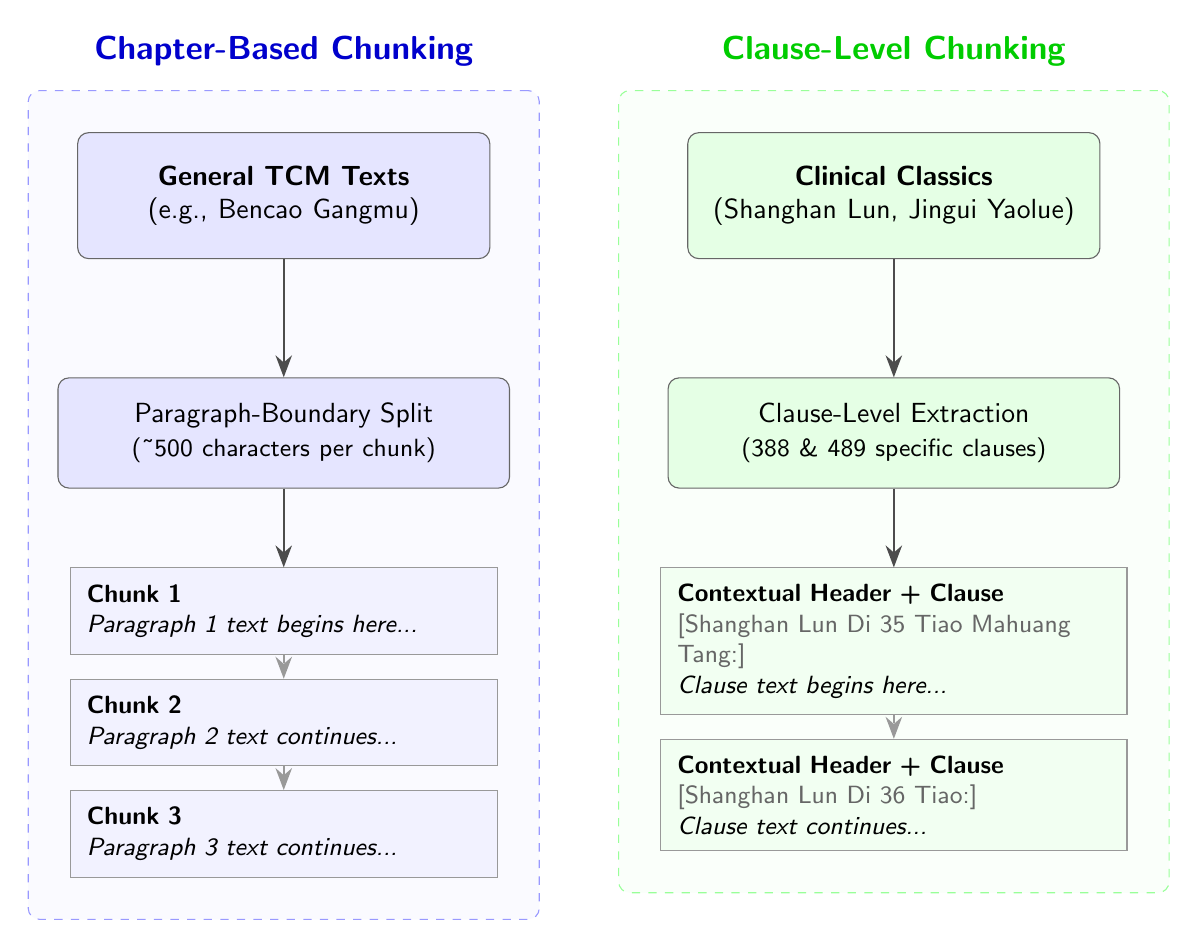
\begin{tikzpicture}[
    node distance=1.5cm and 2cm,
    doc/.style={rectangle, rounded corners, draw=black!60, text width=5cm, align=center, minimum height=1.6cm, font=\sffamily\bfseries},
    process/.style={rectangle, rounded corners, draw=black!60, text width=5.5cm, align=center, minimum height=1.4cm, font=\sffamily},
    chunk/.style={rectangle, draw=black!40, text width=5cm, align=left, minimum height=1.1cm, font=\sffamily\small, inner sep=6pt},
    headerchunk/.style={rectangle, draw=black!40, text width=5.5cm, align=left, minimum height=1.1cm, font=\sffamily\small, inner sep=6pt},
    arrow/.style={-{Stealth[scale=1.2]}, thick, draw=black!70},
    groupbox/.style={rectangle, rounded corners, dashed, inner sep=15pt}
]

\node[doc, fill=blue!10] (doc1) {General TCM Texts\\{\mdseries\normalsize (e.g., Bencao Gangmu)}};

\node[process, fill=blue!10, below=of doc1] (proc1) {Paragraph-Boundary Split\\{\small (\char`\~500 characters per chunk)}};

\node[chunk, fill=blue!5, below=1cm of proc1] (chunk1) {\textbf{Chunk 1}\\ \textit{Paragraph 1 text begins here...}};
\node[chunk, fill=blue!5, below=0.3cm of chunk1] (chunk2) {\textbf{Chunk 2}\\ \textit{Paragraph 2 text continues...}};
\node[chunk, fill=blue!5, below=0.3cm of chunk2] (chunk3) {\textbf{Chunk 3}\\ \textit{Paragraph 3 text continues...}};

\draw[arrow] (doc1) -- (proc1);
\draw[arrow] (proc1) -- (chunk1);
\draw[arrow, dashed, draw=black!40] (chunk1) -- (chunk2);
\draw[arrow, dashed, draw=black!40] (chunk2) -- (chunk3);

\node[doc, fill=green!10, right=2.5cm of doc1] (doc2) {Clinical Classics\\{\mdseries\normalsize (Shanghan Lun, Jingui Yaolue)}};

\node[process, fill=green!10, below=of doc2] (proc2) {Clause-Level Extraction\\{\small (388 \& 489 specific clauses)}};

\node[headerchunk, fill=green!5, below=1cm of proc2] (chunkA) {\textbf{Contextual Header + Clause}\\ \textcolor{black!60}{[Shanghan Lun Di 35 Tiao Mahuang Tang:]}\\ \textit{Clause text begins here...}};
\node[headerchunk, fill=green!5, below=0.3cm of chunkA] (chunkB) {\textbf{Contextual Header + Clause}\\ \textcolor{black!60}{[Shanghan Lun Di 36 Tiao:]}\\ \textit{Clause text continues...}};

\draw[arrow] (doc2) -- (proc2);
\draw[arrow] (proc2) -- (chunkA);
\draw[arrow, dashed, draw=black!40] (chunkA) -- (chunkB);

\begin{scope}[on background layer]
    \node[groupbox, draw=blue!40, fill=blue!2, fit=(doc1) (chunk3)] (bg1) {};
    \node[anchor=south, font=\sffamily\large\bfseries, text=blue!80!black, yshift=5pt] at (bg1.north) {Chapter-Based Chunking};
    \node[groupbox, draw=green!40, fill=green!2, fit=(doc2) (chunkB)] (bg2) {};
    \node[anchor=south, font=\sffamily\large\bfseries, text=green!80!black, yshift=5pt] at (bg2.north) {Clause-Level Chunking};
\end{scope}

\end{tikzpicture}
\caption{Comparison of chunking strategies for different text types.}
\label{fig:chunking_strategy}
\end{figure}

\section{Hybrid Retrieval Architecture}

The retrieval mechanism combines dense vector search with symbolic knowledge graph traversal to achieve high recall and precision.

\subsection{Vector Search and Chronological Boost}

The system uses DashScope text-embedding-v4 (1024 dimensions) for semantic vector search. To handle the large corpus, the retriever initially fetches a broader set of candidates (k $\times$ 3), followed by reranking with the qwen3-rerank cross-encoder model to re-order results by semantic relevance before applying further filtering.

A unique feature of TCM-Sage is the source authority chronological boost. Distance scores are adjusted by a factor of 0.90 to 0.97 based on the historical authority of the text. This boost is topic-dependent rather than a simple linear ranking, ensuring that foundational texts like the \textit{Huangdi Neijing} are prioritized for theoretical queries, while later \textit{Wenbing} texts are favored for febrile disease queries.

\subsection{Formula-Aware Canonical Retrieval}

When the system detects a specific formula name in the user's query, it triggers a metadata-filtered search in canonical texts. This ensures that the primary source for a formula is always included in the context, even if other semantically similar but less authoritative texts are also retrieved.

\subsection{Knowledge Graph and Crosswalk Bridge}

The SymMap 2.0 knowledge graph is traversed using the NetworkX library. Entity matching is performed using the jieba segmentation tool combined with a custom alias map that bridges colloquial modern Chinese terms to their classical equivalents. For example, a user query mentioning a modern symptom name is resolved to its classical counterpart in SymMap, enabling retrieval of related herbs, formulas, and syndromes that would otherwise be missed by vector search alone.

\begin{figure}[H]
    \centering
    \resizebox{\textwidth}{!}{%
    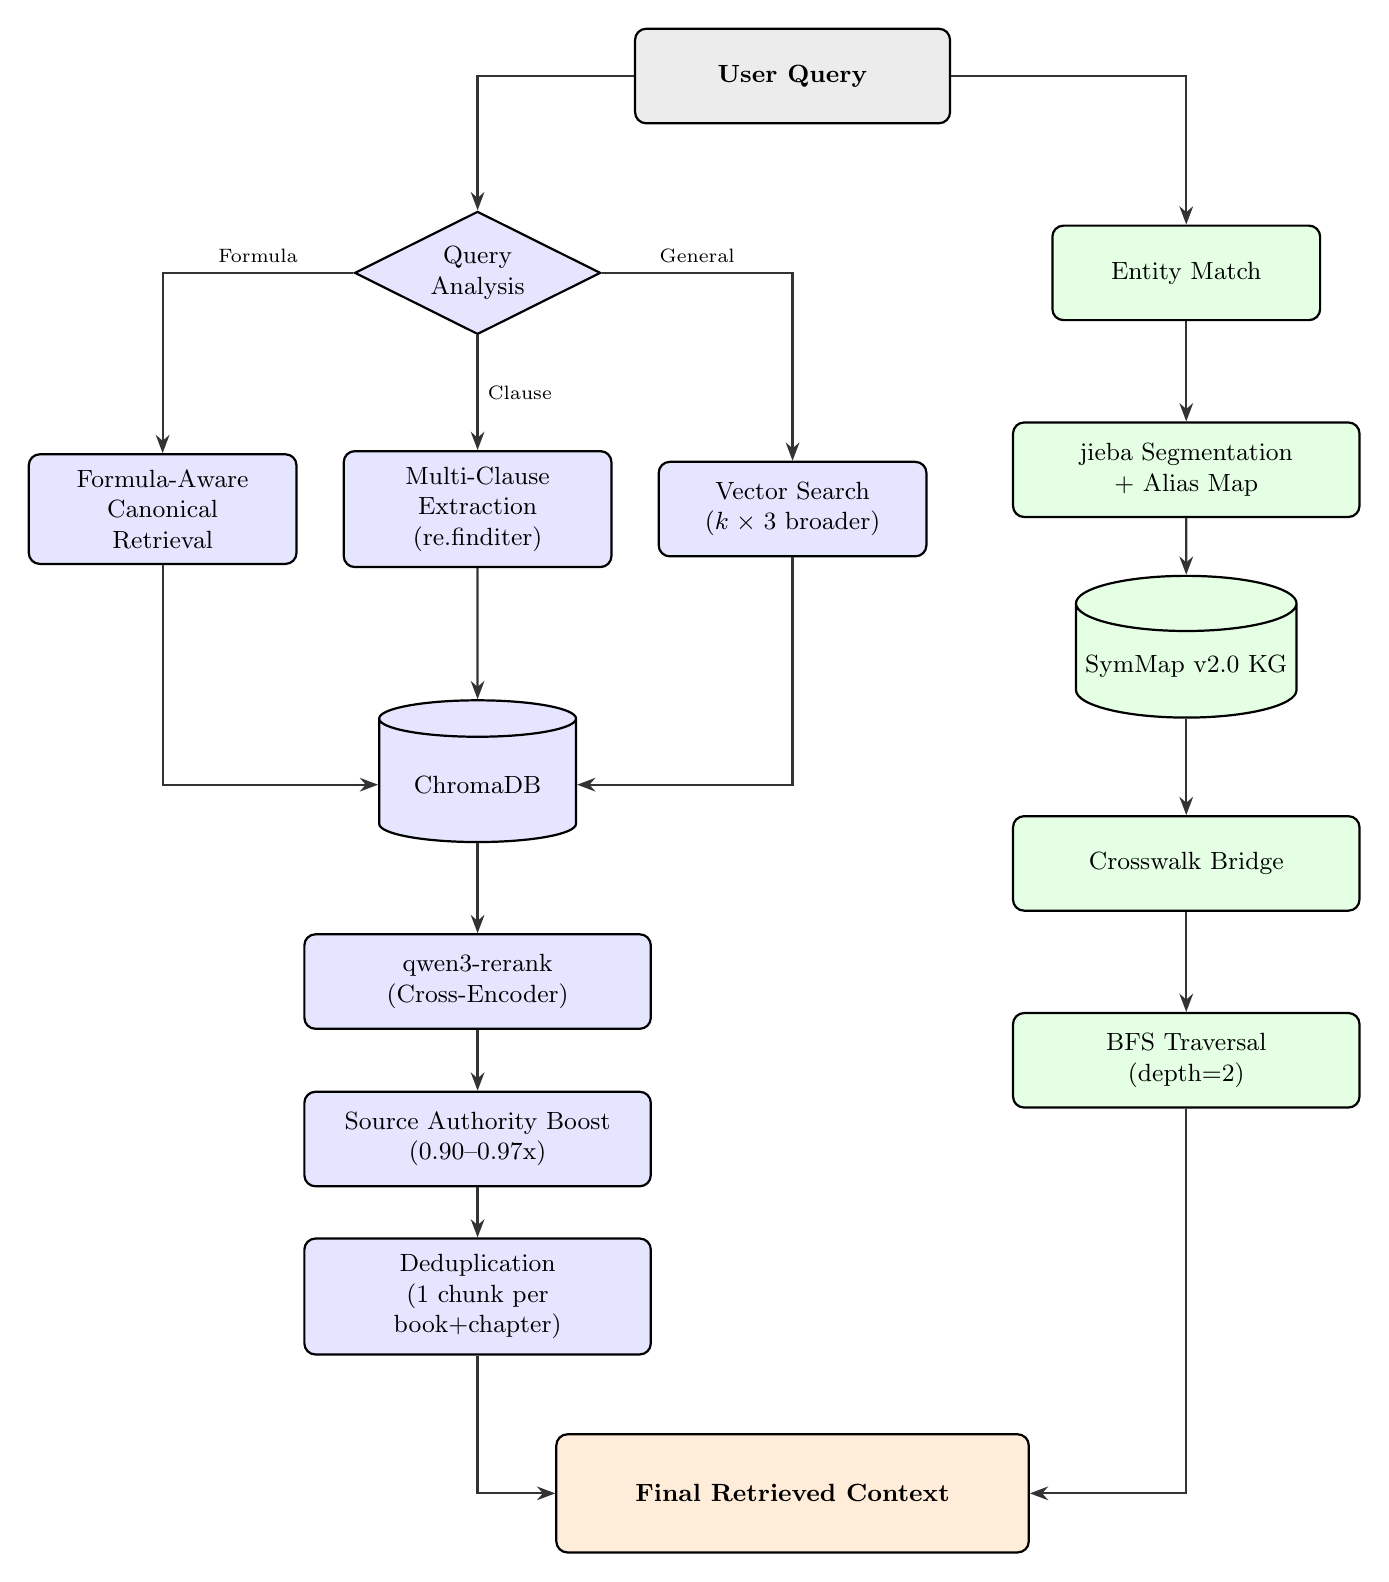
\begin{tikzpicture}[
        >={Stealth[scale=1]},
        base/.style={align=center, draw, thick, font=\small, minimum height=1.2cm},
        process/.style={base, rectangle, rounded corners, inner sep=0.2cm},
        decision/.style={base, diamond, aspect=2, inner sep=0.1cm},
        database/.style={base, cylinder, shape border rotate=90, aspect=0.25, minimum width=2.5cm, minimum height=1.8cm},
        vectorpath/.style={fill=blue!10},
        kgpath/.style={fill=green!10},
        arrow/.style={->, thick, draw=black!80}
    ]

        \node[process, fill=gray!15, minimum width=4cm] (query) at (0, 0) {\textbf{User Query}};

        \node[decision, vectorpath] (qa) at (-4, -2.5) {Query\\Analysis};
        
        \node[process, vectorpath, text width=3cm] (form) at (-8, -5.5) {Formula-Aware\\Canonical\\Retrieval};
        \node[process, vectorpath, text width=3cm] (clause) at (-4, -5.5) {Multi-Clause\\Extraction\\(re.finditer)};
        \node[process, vectorpath, text width=3cm] (gen) at (0, -5.5) {Vector Search\\($k \times 3$ broader)};
        
        \node[database, vectorpath] (chroma) at (-4, -9) {ChromaDB};
        
        \node[process, vectorpath, text width=4cm] (rerank) at (-4, -11.5) {qwen3-rerank\\(Cross-Encoder)};
        \node[process, vectorpath, text width=4cm] (boost) at (-4, -13.5) {Source Authority Boost\\(0.90--0.97x)};
        \node[process, vectorpath, text width=4cm] (dedup) at (-4, -15.5) {Deduplication\\(1 chunk per book+chapter)};

        \node[process, kgpath, text width=3cm] (em) at (5, -2.5) {Entity Match};
        \node[process, kgpath, text width=4cm] (jieba) at (5, -5) {jieba Segmentation\\+ Alias Map};
        \node[database, kgpath] (symmap) at (5, -7.5) {SymMap v2.0 KG};
        \node[process, kgpath, text width=4cm] (crosswalk) at (5, -10) {Crosswalk Bridge};
        \node[process, kgpath, text width=4cm] (bfs) at (5, -12.5) {BFS Traversal\\(depth=2)};

        \node[process, fill=orange!15, minimum width=6cm, minimum height=1.5cm] (final) at (0, -18) {\textbf{Final Retrieved Context}};

        \draw[arrow] (query) -| (qa);
        \draw[arrow] (query) -| (em);

        \draw[arrow] (qa) -| node[above, near start, font=\scriptsize] {Formula} (form);
        \draw[arrow] (qa) -- node[right, font=\scriptsize] {Clause} (clause);
        \draw[arrow] (qa) -| node[above, near start, font=\scriptsize] {General} (gen);

        \draw[arrow] (form) |- (chroma);
        \draw[arrow] (clause) -- (chroma);
        \draw[arrow] (gen) |- (chroma);

        \draw[arrow] (chroma) -- (rerank);
        \draw[arrow] (rerank) -- (boost);
        \draw[arrow] (boost) -- (dedup);

        \draw[arrow] (em) -- (jieba);
        \draw[arrow] (jieba) -- (symmap);
        \draw[arrow] (symmap) -- (crosswalk);
        \draw[arrow] (crosswalk) -- (bfs);

        \draw[arrow] (dedup) |- (final);
        \draw[arrow] (bfs) |- (final);

    \end{tikzpicture}}
    \caption{The hybrid retrieval pipeline combining vector and graph-based methods.}
    \label{fig:retrieval_flow}
\end{figure}

\section{Generation Pipeline}

The generation pipeline synthesizes the retrieved context into a coherent, evidence-backed response. The system supports eight LLM providers (DashScope/Alibaba, OpenAI, Anthropic, Google, OpenRouter, Together, Ollama, and LMStudio), allowing deployment across cloud and local configurations. Each provider is accessed through a unified \texttt{create\_llm()} factory function.

\subsection{Query Classification and Temperature Control}

Before generation, a dedicated classifier LLM (running at temperature 0.0 for deterministic output) categorizes each query as either \textit{informational} (general knowledge, definitions, explanations) or \textit{prescriptive} (diagnoses, treatments, formula recommendations). This classification determines the generation temperature:

\begin{itemize}
    \item \textbf{Informational:} Temperature 0.7 --- allows natural language generation for educational explanations.
    \item \textbf{Prescriptive:} Temperature 0.0 --- maximizes precision and reproducibility for clinical queries where accuracy is critical.
\end{itemize}

This dual-temperature design reflects a safety-conscious approach: clinical queries demand the highest possible fidelity to source material, while general knowledge queries benefit from slightly more natural language generation.

\subsection{System Prompt and Framework}

The system prompt is structured around the "Bian Zheng Lun Zhi" (Pattern Differentiation and Treatment) framework and the "Yuan Liu" (Source and Development) methodology. It includes specific instructions for "Jun Chen Zuo Shi" (Sovereign, Minister, Assistant, and Courier) drug analysis for formulas.

\subsection{Post-Context Instruction Anchoring}

To prevent the model from ignoring formatting rules, TCM-Sage uses post-context instruction anchoring. Formatting instructions are placed after the retrieved context rather than before it. This ensures that the model's final attention is focused on the required output structure.

\subsection{Pattern Priming and User Intent}

The system employs "Pattern Priming" by providing the retrieved context in a structured markdown format (using headers and blockquotes). This encourages the LLM to produce similarly structured outputs. An ancient measurement conversion table is embedded in the prompt to ensure accurate dosage translations. Finally, a "User Intent Priority" block ensures that specific user preferences always override default formatting rules.

\section{Arena Evaluation Design}

The evaluation system is inspired by the LMSYS Chatbot Arena, providing a blind A/B testing framework for TCM practitioners.

\subsection{Blind A/B Testing}

The system compares the full TCM-Sage pipeline (RAG system) against a plain LLM baseline. The baseline model is given a generic "helpful assistant" prompt and access to a standard web search tool (DuckDuckGo). Both systems stream their responses simultaneously using Server-Sent Events (SSE), with their positions (Left vs. Right) randomly assigned to eliminate position bias.

\subsection{Statistical Validation}

The results of the arena votes are analyzed using a paired t-test and Cohen's $d$ effect size. These metrics provide statistical proof of the RAG system's effectiveness. The t-test determines if the improvement is due to the system's design rather than random chance, while Cohen's $d$ quantifies the magnitude of the improvement.

\begin{figure}[H]
    \centering
    \resizebox{0.85\textwidth}{!}{%
    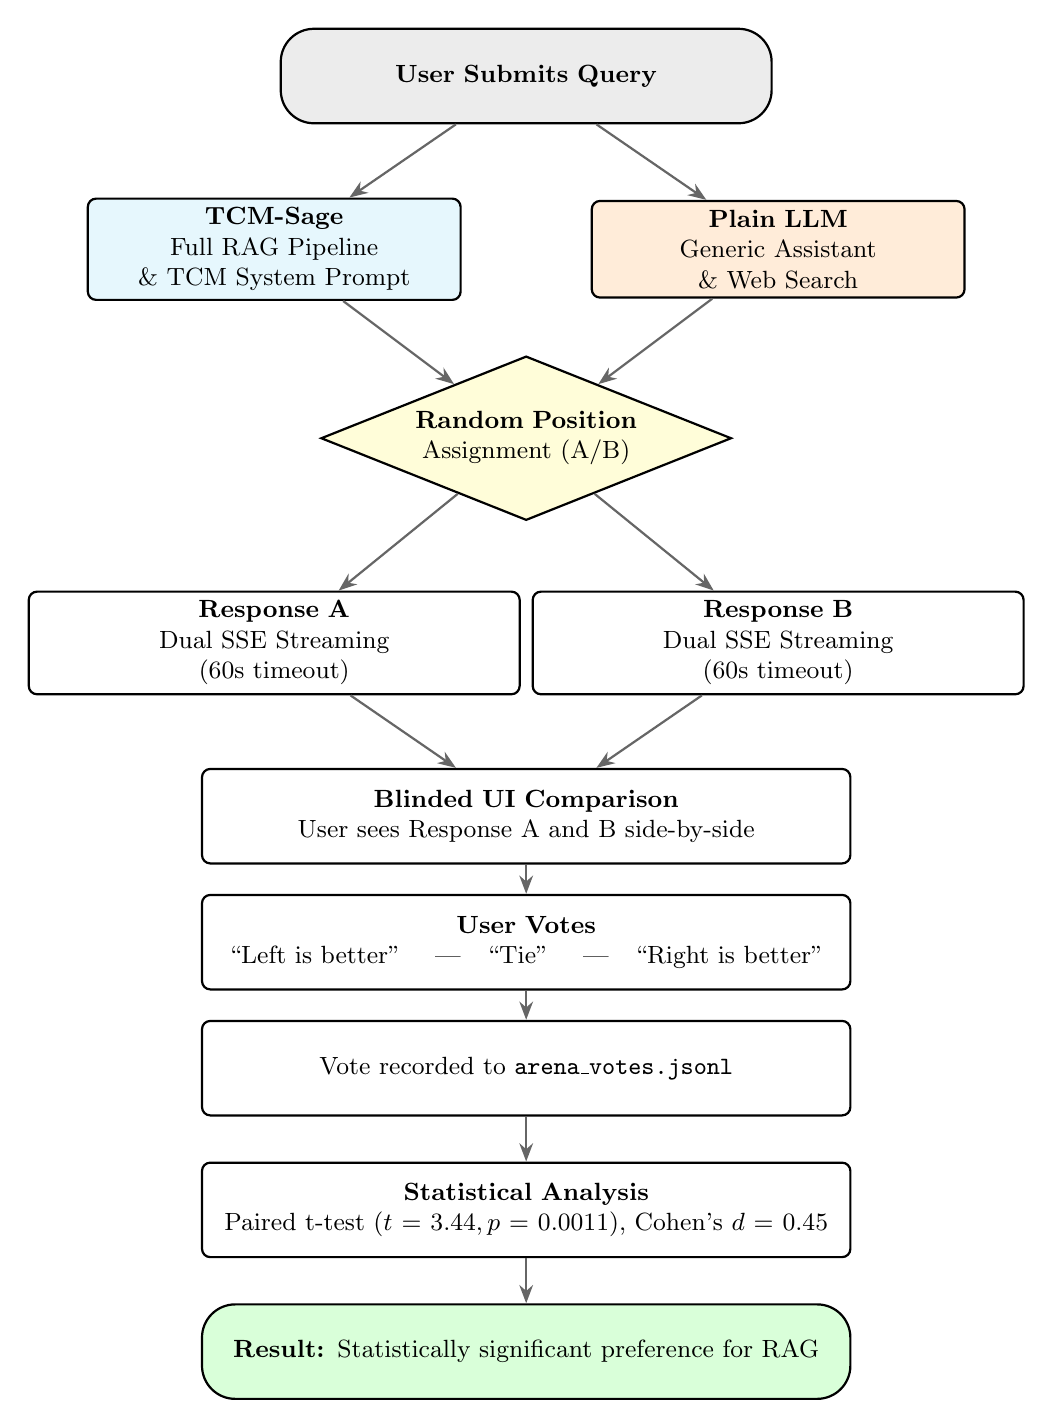
\begin{tikzpicture}[
        base/.style={draw, align=center, minimum height=1.2cm, thick, font=\small},
        start/.style={base, rectangle, rounded corners=12pt, fill=gray!15, text width=6cm},
        process/.style={base, rectangle, rounded corners=3pt, fill=white, text width=6cm},
        tcm/.style={process, fill=cyan!10, text width=4.5cm},
        llm/.style={process, fill=orange!15, text width=4.5cm},
        decision/.style={base, diamond, aspect=2.5, fill=yellow!15, text width=3.5cm, inner sep=0pt},
        arrow/.style={->, >={Stealth[scale=1]}, thick, draw=gray!80!black}
    ]
    
    \node (query) at (0, 0) [start] {\textbf{User Submits Query}};
    
    \node (tcm) at (-3.2, -2.2) [tcm] {\textbf{TCM-Sage}\\Full RAG Pipeline\\\& TCM System Prompt};
    \node (plain) at (3.2, -2.2) [llm] {\textbf{Plain LLM}\\Generic Assistant\\\& Web Search};
    
    \node (random) at (0, -4.6) [decision] {\textbf{Random Position}\\Assignment (A/B)};
    
    \node (streamA) at (-3.2, -7.2) [process] {\textbf{Response A}\\Dual SSE Streaming\\(60s timeout)};
    \node (streamB) at (3.2, -7.2) [process] {\textbf{Response B}\\Dual SSE Streaming\\(60s timeout)};
    
    \node (ui) at (0, -9.4) [process, text width=8cm] {\textbf{Blinded UI Comparison}\\User sees Response A and B side-by-side};
    
    \node (vote) at (0, -11) [process, text width=8cm] {\textbf{User Votes}\\``Left is better'' \quad|\quad ``Tie'' \quad|\quad ``Right is better''};
    
    \node (json) at (0, -12.6) [process, text width=8cm] {Vote recorded to \texttt{arena\_votes.jsonl}};
    
    \node (stats) at (0, -14.4) [process, text width=8cm] {\textbf{Statistical Analysis}\\Paired t-test ($t=3.44, p=0.0011$), Cohen's $d=0.45$};
    
    \node (result) at (0, -16.2) [start, fill=green!15, text width=8cm] {\textbf{Result:} Statistically significant preference for RAG};
    
    \draw [arrow] (query) -- (tcm);
    \draw [arrow] (query) -- (plain);
    \draw [arrow] (tcm) -- (random);
    \draw [arrow] (plain) -- (random);
    \draw [arrow] (random) -- (streamA);
    \draw [arrow] (random) -- (streamB);
    \draw [arrow] (streamA) -- (ui);
    \draw [arrow] (streamB) -- (ui);
    \draw [arrow] (ui) -- (vote);
    \draw [arrow] (vote) -- (json);
    \draw [arrow] (json) -- (stats);
    \draw [arrow] (stats) -- (result);
    
    \end{tikzpicture}}
    \caption{The blind A/B Arena evaluation and statistical validation flow.}
    \label{fig:arena_flow}
\end{figure}


\chapter{Technical Implementation}
\label{ch:implementation}

This chapter details the technical architecture and implementation of the TCM-Sage system. The implementation focuses on three core pillars: a retrieval-augmented generation (RAG) pipeline optimized for classical Traditional Chinese Medicine (TCM) texts, a knowledge graph (KG) integration for structured entity resolution, and a blind A/B evaluation framework (Arena) for performance benchmarking.

\section{Technology Stack}

The system is built on a full-stack architecture with the following components:

\subsection{Backend Infrastructure}
The backend is implemented using \textbf{Python 3.13}, utilizing the \textbf{FastAPI} framework for high-concurrency asynchronous API handling. The core orchestration layer uses \textbf{LangChain}, which provides the abstraction for retrieval chains and prompt templates. Data persistence for vectorized text is managed by \textbf{ChromaDB}, an open-source vector database chosen for its local persistence capabilities and efficient metadata filtering.

\subsection{Frontend and User Interface}
The user interface is developed with \textbf{Next.js 16} (App Router) and \textbf{React 19}. \textbf{TypeScript} ensures type safety across the application, while \textbf{Tailwind CSS} is used for responsive, utility-first styling. The interface supports a dual-stream architecture for the Arena evaluation system, allowing simultaneous rendering of two independent Large Language Model (LLM) responses.

\subsection{Language Models and Embeddings}
\begin{itemize}
    \item \textbf{LLM:} The system utilizes the \textbf{DashScope API} (Qwen series), specifically targeting the international endpoint (\texttt{dashscope-intl.aliyuncs.com}) for consistent availability.
    \item \textbf{Embedding Model:} \textbf{DashScope text-embedding-v4} (1024 dimensions) with TCM domain-specific asymmetric prefixes. Ingestion uses the prefix ``Generate semantic representation for this classical TCM text for retrieval'' while queries use ``Generate semantic representation for this TCM clinical question to retrieve relevant classical passages.'' This asymmetric strategy follows DashScope best practices for domain-specific retrieval.
    \item \textbf{Reranker:} \textbf{qwen3-rerank} cross-encoder, wired into the \texttt{hybrid\_search()} pipeline. The reranker operates on vector search results \textit{before} combining with knowledge graph results, as KG facts (structured entity relationships) do not benefit from semantic reranking. Both the original distance score and the reranker's relevance score are preserved in metadata for downstream use.
\end{itemize}

\subsection{Knowledge Graph and Local Support}
The structural backbone for entity resolution is \textbf{SymMap v2.0}, implemented using the \textbf{NetworkX} library. A custom \textit{crosswalk bridge} was developed to map colloquial and modern medical terms to classical TCM entities. For researchers requiring local privacy, the system supports local LLM deployment via \textbf{Ollama} and \textbf{LMStudio} through standard OpenAI-compatible endpoints.

\section{Data Acquisition and Preprocessing}

The quality of a RAG system is fundamentally bounded by its underlying corpus. TCM-Sage utilizes a curated set of 17 classical TCM texts, totaling 3.72 million characters in UTF-8 encoding.

\subsection{Chunking Strategies}
To preserve the semantic integrity of classical texts, two distinct chunking strategies were implemented:
\begin{enumerate}
    \item \textbf{Chapter-based Chunking:} Applied to the majority of the corpus, where texts are split by \textit{Pianming} (chapter title) markers. This results in an average chunk size of approximately 500 characters, providing sufficient context for general theoretical queries.
    \item \textbf{Clause-level Chunking:} Specifically for \textit{Shanghan Lun} (388 clauses) and \textit{Jingui Yaolue} (489 clauses). Using regex pattern matching on numerical markers (e.g., "N."), the system extracts individual clinical clauses. This granularity is essential for formula-based retrieval where specific symptom-sign clusters are defined within a single clause.
\end{enumerate}

\subsection{Contextual Header Prepend}
To improve embedding quality and retrieval precision, each chunk is prepended with a \textit{Contextual Header}. For example, a clause from \textit{Shanghan Lun} is transformed into: \texttt{"<Shanghan Lun> Clause 35 Mahuang Tang: [Clause Content]"}. This ensures that even if the clause text itself is brief, the vector representation captures the source book and the associated formula name.

\subsection{Ingestion and Storage}
The ingestion pipeline handles the DashScope batch limit of 10 embeddings per API call through a robust checkpoint/resume system. This prevents data loss during network interruptions or API rate limiting. The final processed corpus consists of 12,204 chunks, requiring approximately 850MB of \textbf{ChromaDB} persistent storage.

\section{Retrieval Pipeline Implementation}

The retrieval pipeline is engineered to address the specific nuances of classical TCM literature, where source authority and formula-specific contexts are paramount.

\subsection{Formula-Aware Canonical Retrieval}
Standard vector search often fails to prioritize the \textit{source} text of a formula. We implemented a specialized detection layer:
\begin{enumerate}
    \item Detect formula names (e.g., \textit{Guizhi Tang}) in the user query.
    \item Perform a metadata-filtered ChromaDB search restricted to canonical texts (\textit{Shanghan Lun} and \textit{Jingui Yaolue}).
    \item Prepend these canonical results to the general retrieval list, ensuring the "original" definition is always present in the context.
\end{enumerate}

\subsection{Multi-Clause Comparison}
TCM practitioners frequently compare different clauses to differentiate syndromes. The system implements an \texttt{extract\_clause\_references} function using \texttt{re.finditer}. It supports various citation formats (with or without "Section" or "Clause" markers) and can retrieve multiple non-contiguous clauses in a single query.

\subsection{Source Authority Boost}
A \textit{Source Chronological Boost} (\texttt{\_SOURCE\_CHRONOLOGICAL\_BOOST}) dictionary applies multipliers (ranging from 0.90 to 0.97) to the distance scores of older, more authoritative texts. This mathematically "pulls" foundational Han Dynasty texts closer to the query than later, more verbose Ming or Qing Dynasty commentaries.

\subsection{Deduplication and Filtering}
To maximize the diversity of information within the context window:
\begin{itemize}
    \item \textbf{Broader Retrieval:} The system initially retrieves $k \times 3$ results before truncation.
    \item \textbf{Source Deduplication:} Only the most relevant chunk per \textit{book + chapter} combination is retained, preventing the LLM from being overwhelmed by repetitive content from a single source.
    \item \textbf{ChromaDB Filters:} Complex filtering uses the \texttt{\$and} operator (e.g., \texttt{'\$and': [\{'clause\_number': num\}, \{'book': name\}]}), as flat dictionaries are ignored by the ChromaDB filter parser.
\end{itemize}

\section{Knowledge Graph Integration}

The SymMap v2.0 knowledge graph provides a structured layer of medical knowledge that complements the unstructured text retrieval.

\subsection{Graph Architecture}
The graph contains 18,450 entities and 21,476 relationships. Key entity types include \textit{Herbs}, \textit{Symptoms}, \textit{TCM Syndromes} (Zheng), and \textit{Modern Diseases}.

\subsection{Entity Matching and Crosswalk}
Mapping modern user queries to classical graph entities is achieved through:
\begin{itemize}
    \item \textbf{Jieba Segmentation:} Tokenizing the query into candidate medical terms.
    \item \textbf{Alias Mapping:} A crosswalk bridge that translates colloquial modern Chinese terms to formal TCM terminology (e.g., ``du zi teng'' [belly ache] $\rightarrow$ ``fu tong'' [abdominal pain], ``shui bu zhao'' [can't sleep] $\rightarrow$ ``shi mian'' [insomnia]).
    \item \textbf{BFS Traversal:} Upon matching an entity, the system performs a Breadth-First Search (BFS) with configurable depth (default 2) to retrieve related symptoms or herbs, providing the LLM with structured diagnostic relationships.
\end{itemize}

\section{Generation and Prompt Engineering}

The generation layer is optimized to ensure the LLM adheres to professional TCM methodologies while maintaining strict formatting. The system supports eight LLM providers through a unified \texttt{create\_llm()} factory function, enabling seamless switching between cloud APIs (DashScope, OpenAI, Anthropic, Google, OpenRouter, Together) and local inference (Ollama, LMStudio).

\subsection{Query Classification}
Each incoming query is first classified by a dedicated classifier LLM (temperature 0.0) into \texttt{informational} or \texttt{prescriptive} categories using \texttt{get\_query\_severity()}. The classification determines which pre-initialized LLM instance handles the query:

\begin{itemize}
    \item \texttt{llm\_informational}: temperature 0.7 for general knowledge queries
    \item \texttt{llm\_prescriptive}: temperature 0.0 for clinical/formula queries
\end{itemize}

The classifier, main LLMs, and verifier can each be configured with independent providers and models via environment variables, allowing fine-grained control over cost and quality trade-offs.

\subsection{System Prompt Architecture}
We use \texttt{ChatPromptTemplate.from\_messages()} to maintain a clean separation between the \texttt{SystemMessage} and the \texttt{UserMessage}. Empirical testing showed that merging these into a single string caused the model to ignore complex formatting constraints.

The \texttt{DEFAULT\_SYSTEM\_PROMPT} incorporates several professional frameworks:
\begin{itemize}
    \item \textbf{Bian Zheng Lun Zhi:} Standard diagnostic and treatment framework.
    \item \textbf{Yuanliu Methodology:} Tracing the origin and evolution of formulas across different sources.
    \item \textbf{Jun Chen Zuo Shi:} Drug hierarchy analysis (Sovereign, Minister, Assistant, Courier).
    \item \textbf{Measurement Conversion:} A hard-coded Han Dynasty conversion table (1 \textit{liang} $\approx$ 13.8g), correcting the common LLM hallucination of 1 \textit{liang} $\approx$ 3g.
\end{itemize}

\subsection{Context Anchoring and Pattern Priming}
To prevent ``context drift,'' we use a boundary marker (\texttt{=== End of References ===}) followed by a \texttt{[Formatting Requirements]} section placed \textit{after} the retrieved context. This ``post-context anchoring'' ensures the most recent tokens the LLM sees are the instructions, not the data. Furthermore, we discovered \textit{Pattern Priming}: by formatting the RAG context as clean Markdown (using headers and blockquotes), the LLM naturally mirrors this structured output format without explicit instruction.

\section{Arena Evaluation System}

To provide an objective measure of RAG effectiveness, we implemented a blind A/B testing framework in \texttt{arena.py}.

\subsection{Baseline Configuration}
The ``Plain LLM'' baseline uses a generic ``helpful assistant'' prompt and has access to \textbf{DuckDuckGo Search} (\texttt{ddgs} package) to simulate a general-purpose AI's ability to retrieve information from the web. This represents a representative general-purpose configuration for non-specialized models.

\subsection{Asynchronous Dual Streaming}
The system uses \texttt{asyncio.Queue} and \texttt{asyncio.gather} to stream responses from both the TCM-Sage pipeline and the baseline simultaneously. A random position assignment (A/B) ensures voters cannot identify the system by its position on the screen.

\subsection{Reliability and Storage}
A 60-second timeout per stream prevents the UI from hanging if one backend fails. All interaction data, including the query, both responses, and the final vote, are stored in a \textbf{JSONL} format with timestamps for later statistical analysis.

\section{Web Application Implementation}

The frontend is designed to be a professional clinical tool, prioritizing clarity and traceability.

\subsection{Internationalization and State}
The system supports Traditional Chinese (default), Simplified Chinese, and English. Language state is managed via \textbf{React Context}, with translations loaded from static JSON files.

\subsection{UX Enhancements}
\begin{itemize}
    \item \textbf{Smart Auto-scroll:} The chat interface automatically scrolls with new content but "unlocks" if the user manually scrolls up to read previous messages, showing a floating "down" button for quick return.
    \item \textbf{Citation Panel:} Clicking a citation number opens a side panel displaying the full source text and a mini knowledge graph view (built with xyflow/React Flow) showing the entity and its immediate relationships.
    \item \textbf{KG Explorer:} A dedicated \texttt{/kg/[entityId]} route provides a full-page \textbf{Cytoscape.js} graph explorer, allowing users to browse the knowledge graph, expand nodes on click, and search for specific entities.
\end{itemize}

\begin{figure}[H]
\centering
\begin{minipage}{0.48\textwidth}
    \centering
    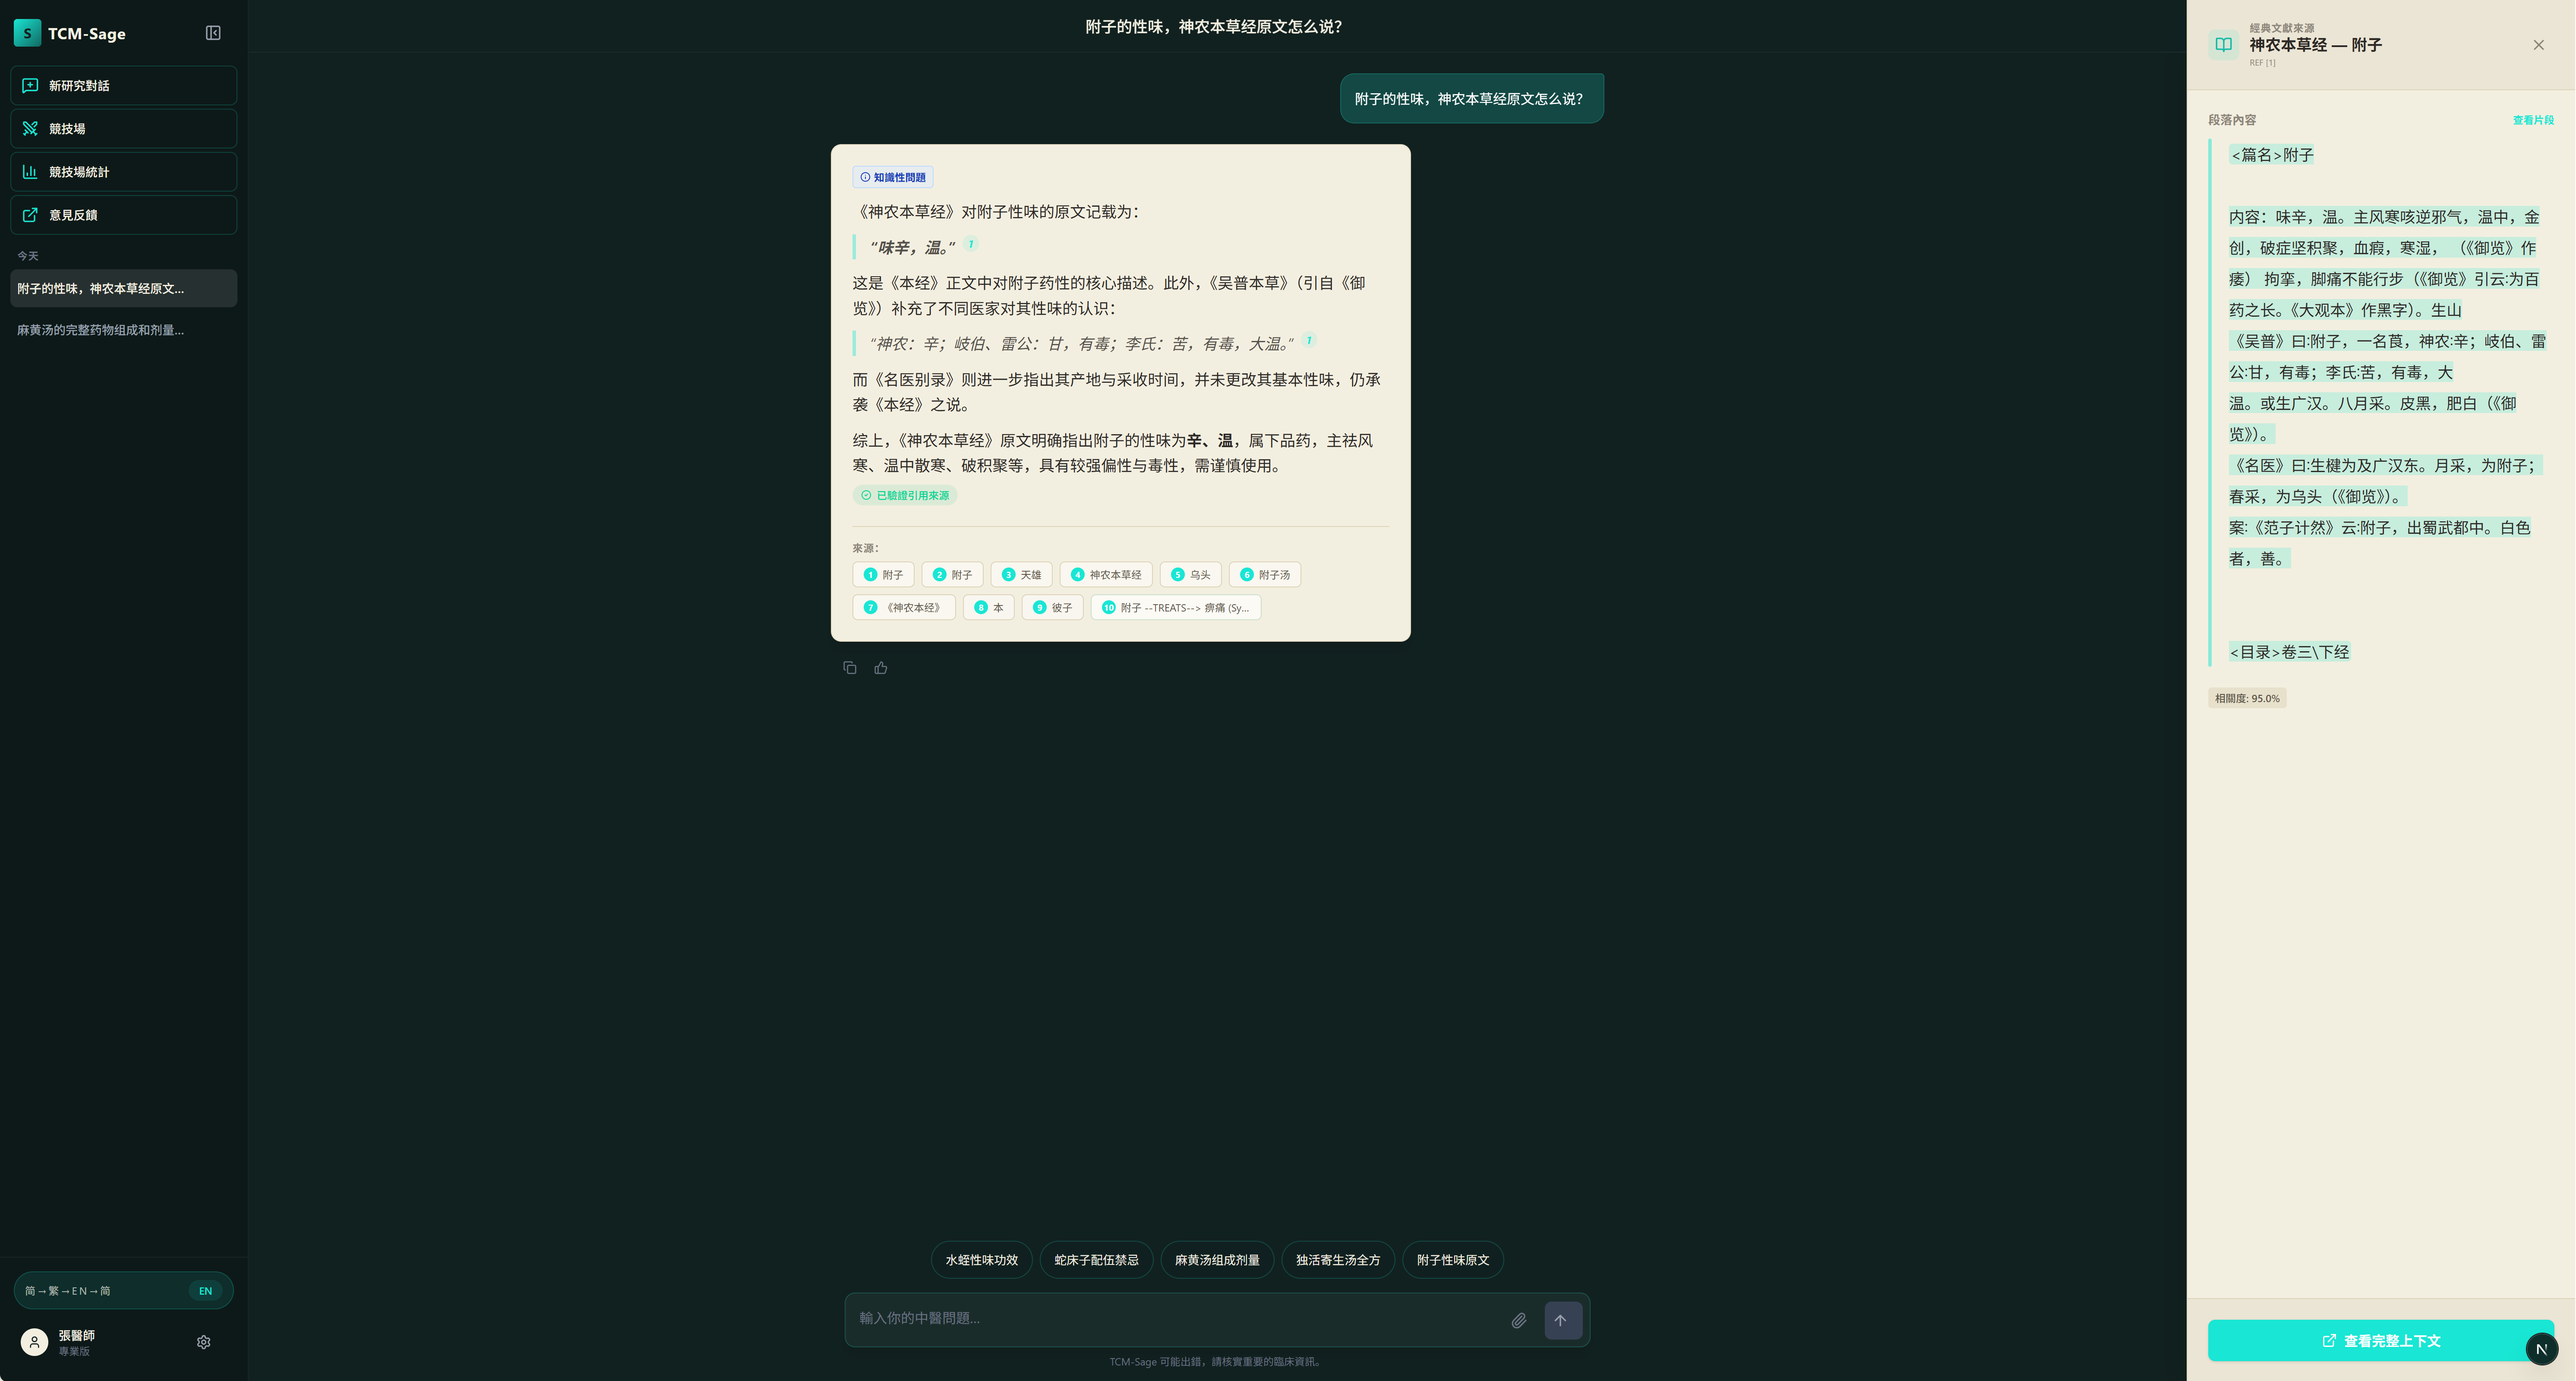
\includegraphics[width=\textwidth]{figures/ui-main-chat.png}
    \caption{Citation Panel showing the original source text with click-through to full passage.}
    \label{fig:ui_main}
\end{minipage}\hfill
\begin{minipage}{0.48\textwidth}
    \centering
    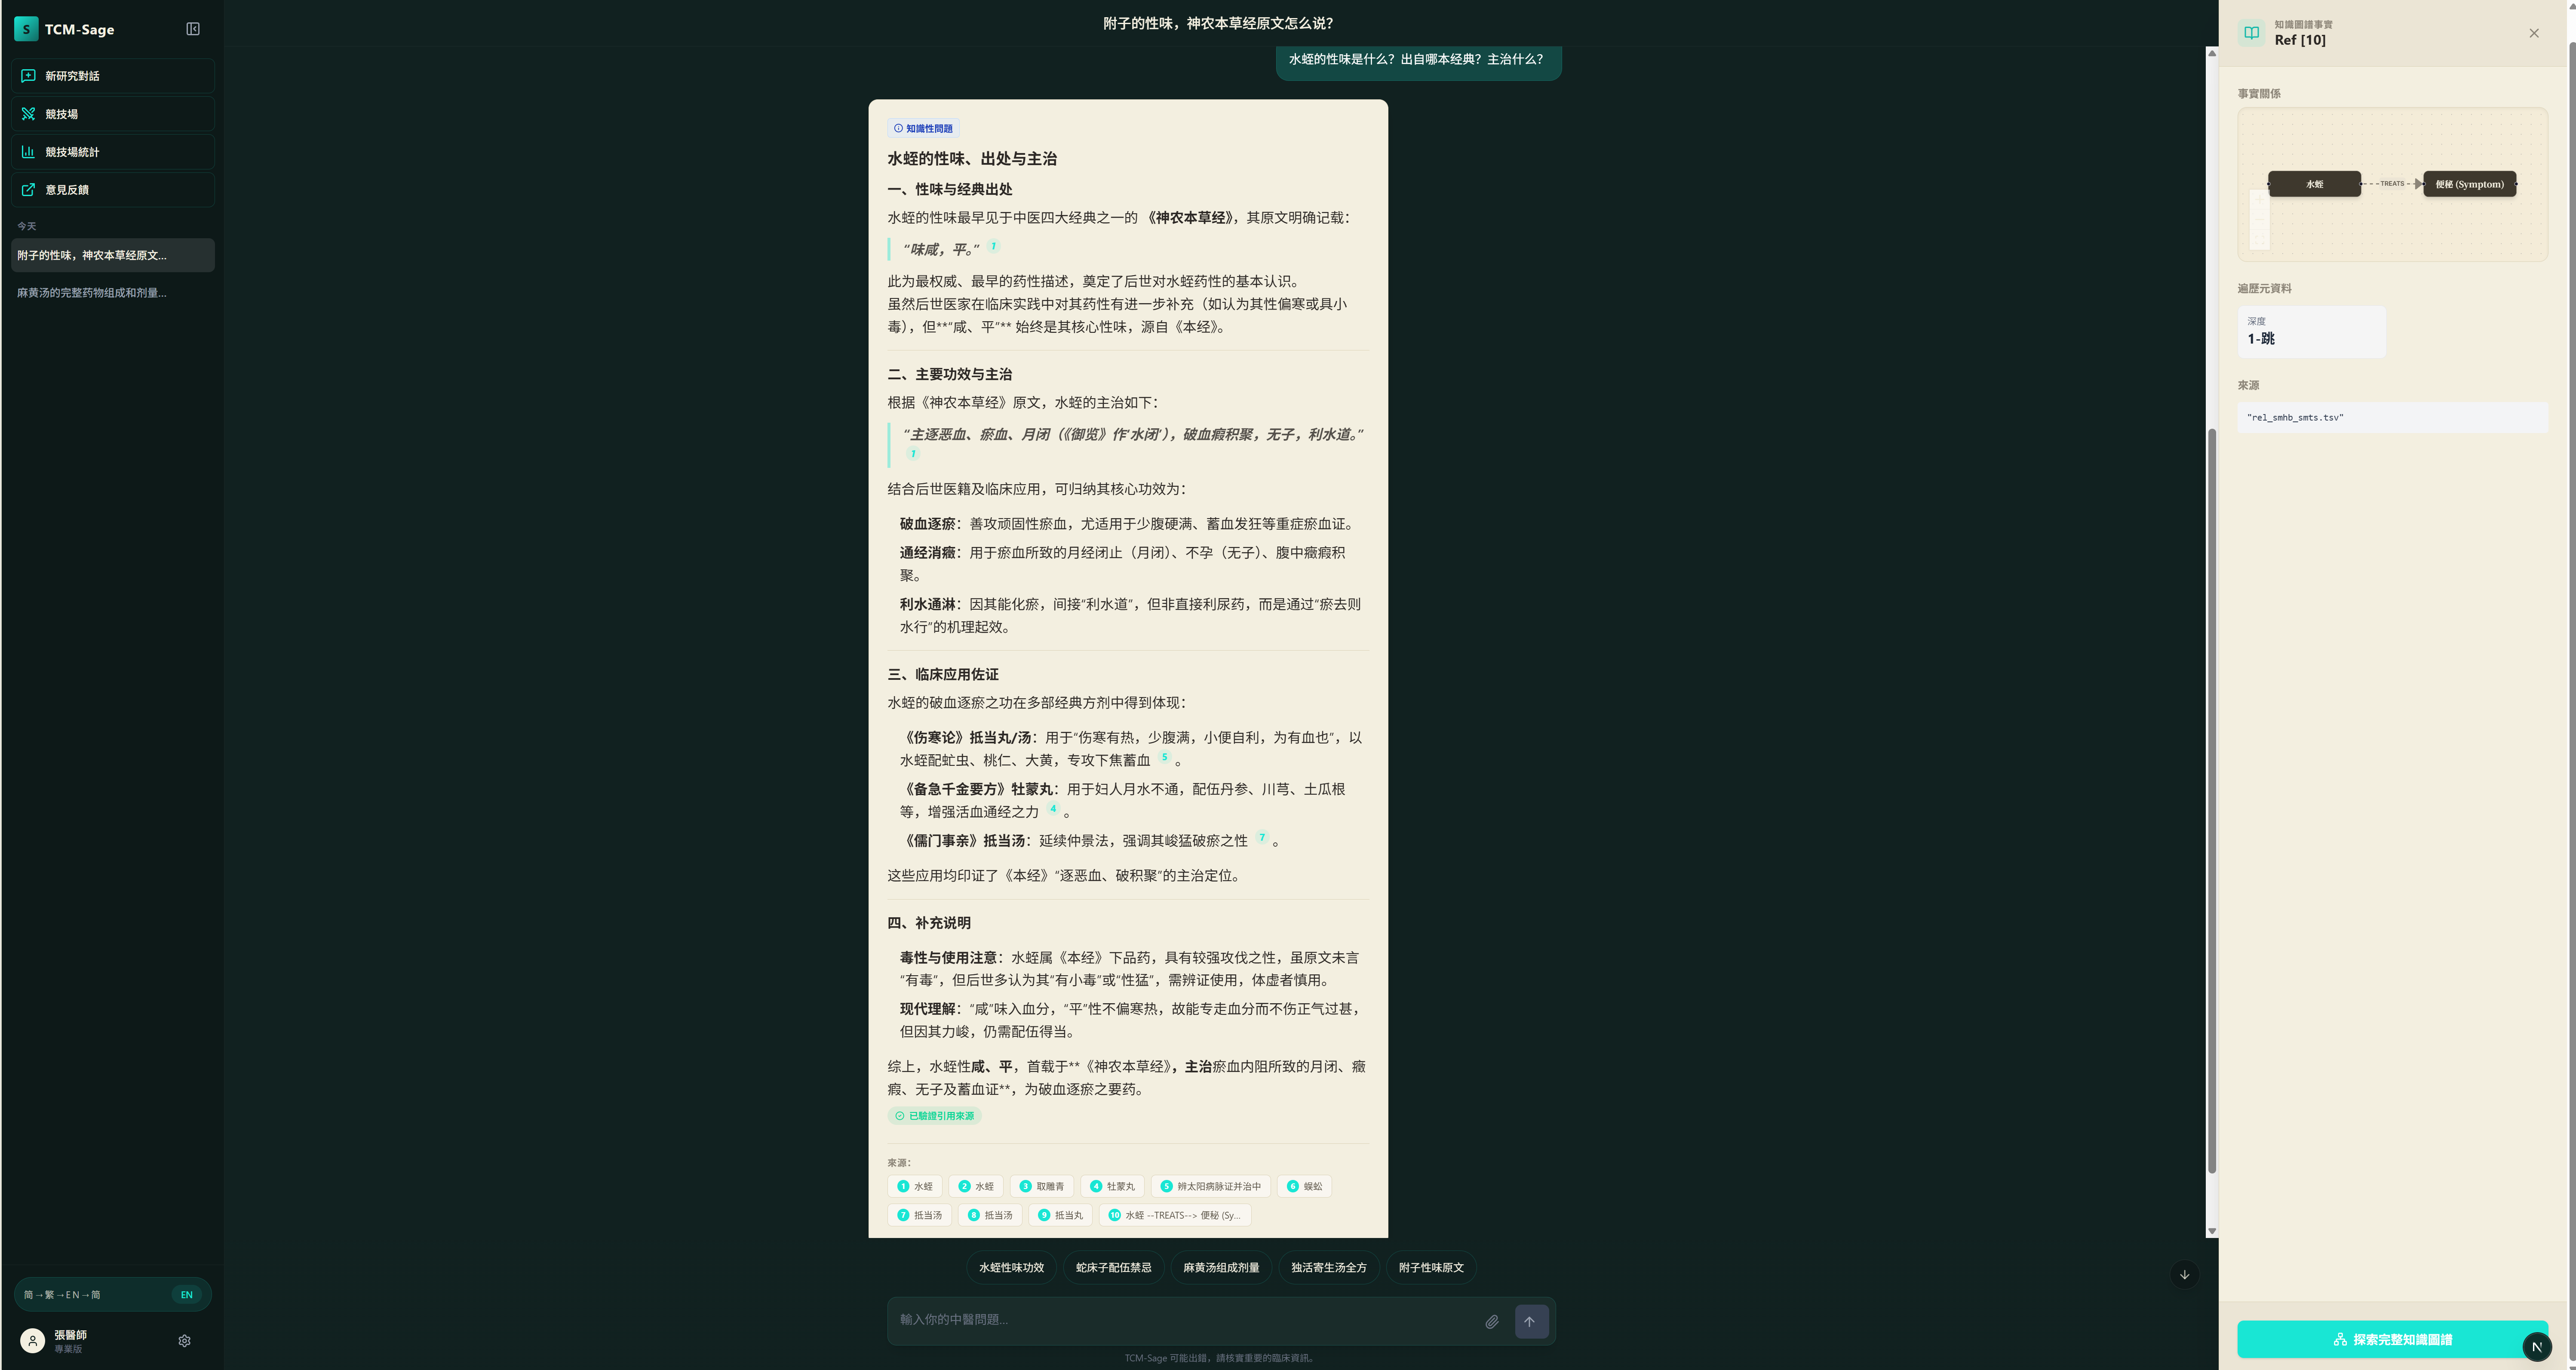
\includegraphics[width=\textwidth]{figures/ui-kg-main-chat.png}
    \caption{Citation Panel showing the mini knowledge graph view for an entity.}
    \label{fig:ui_kg_cite}
\end{minipage}
\end{figure}

\begin{figure}[H]
\centering
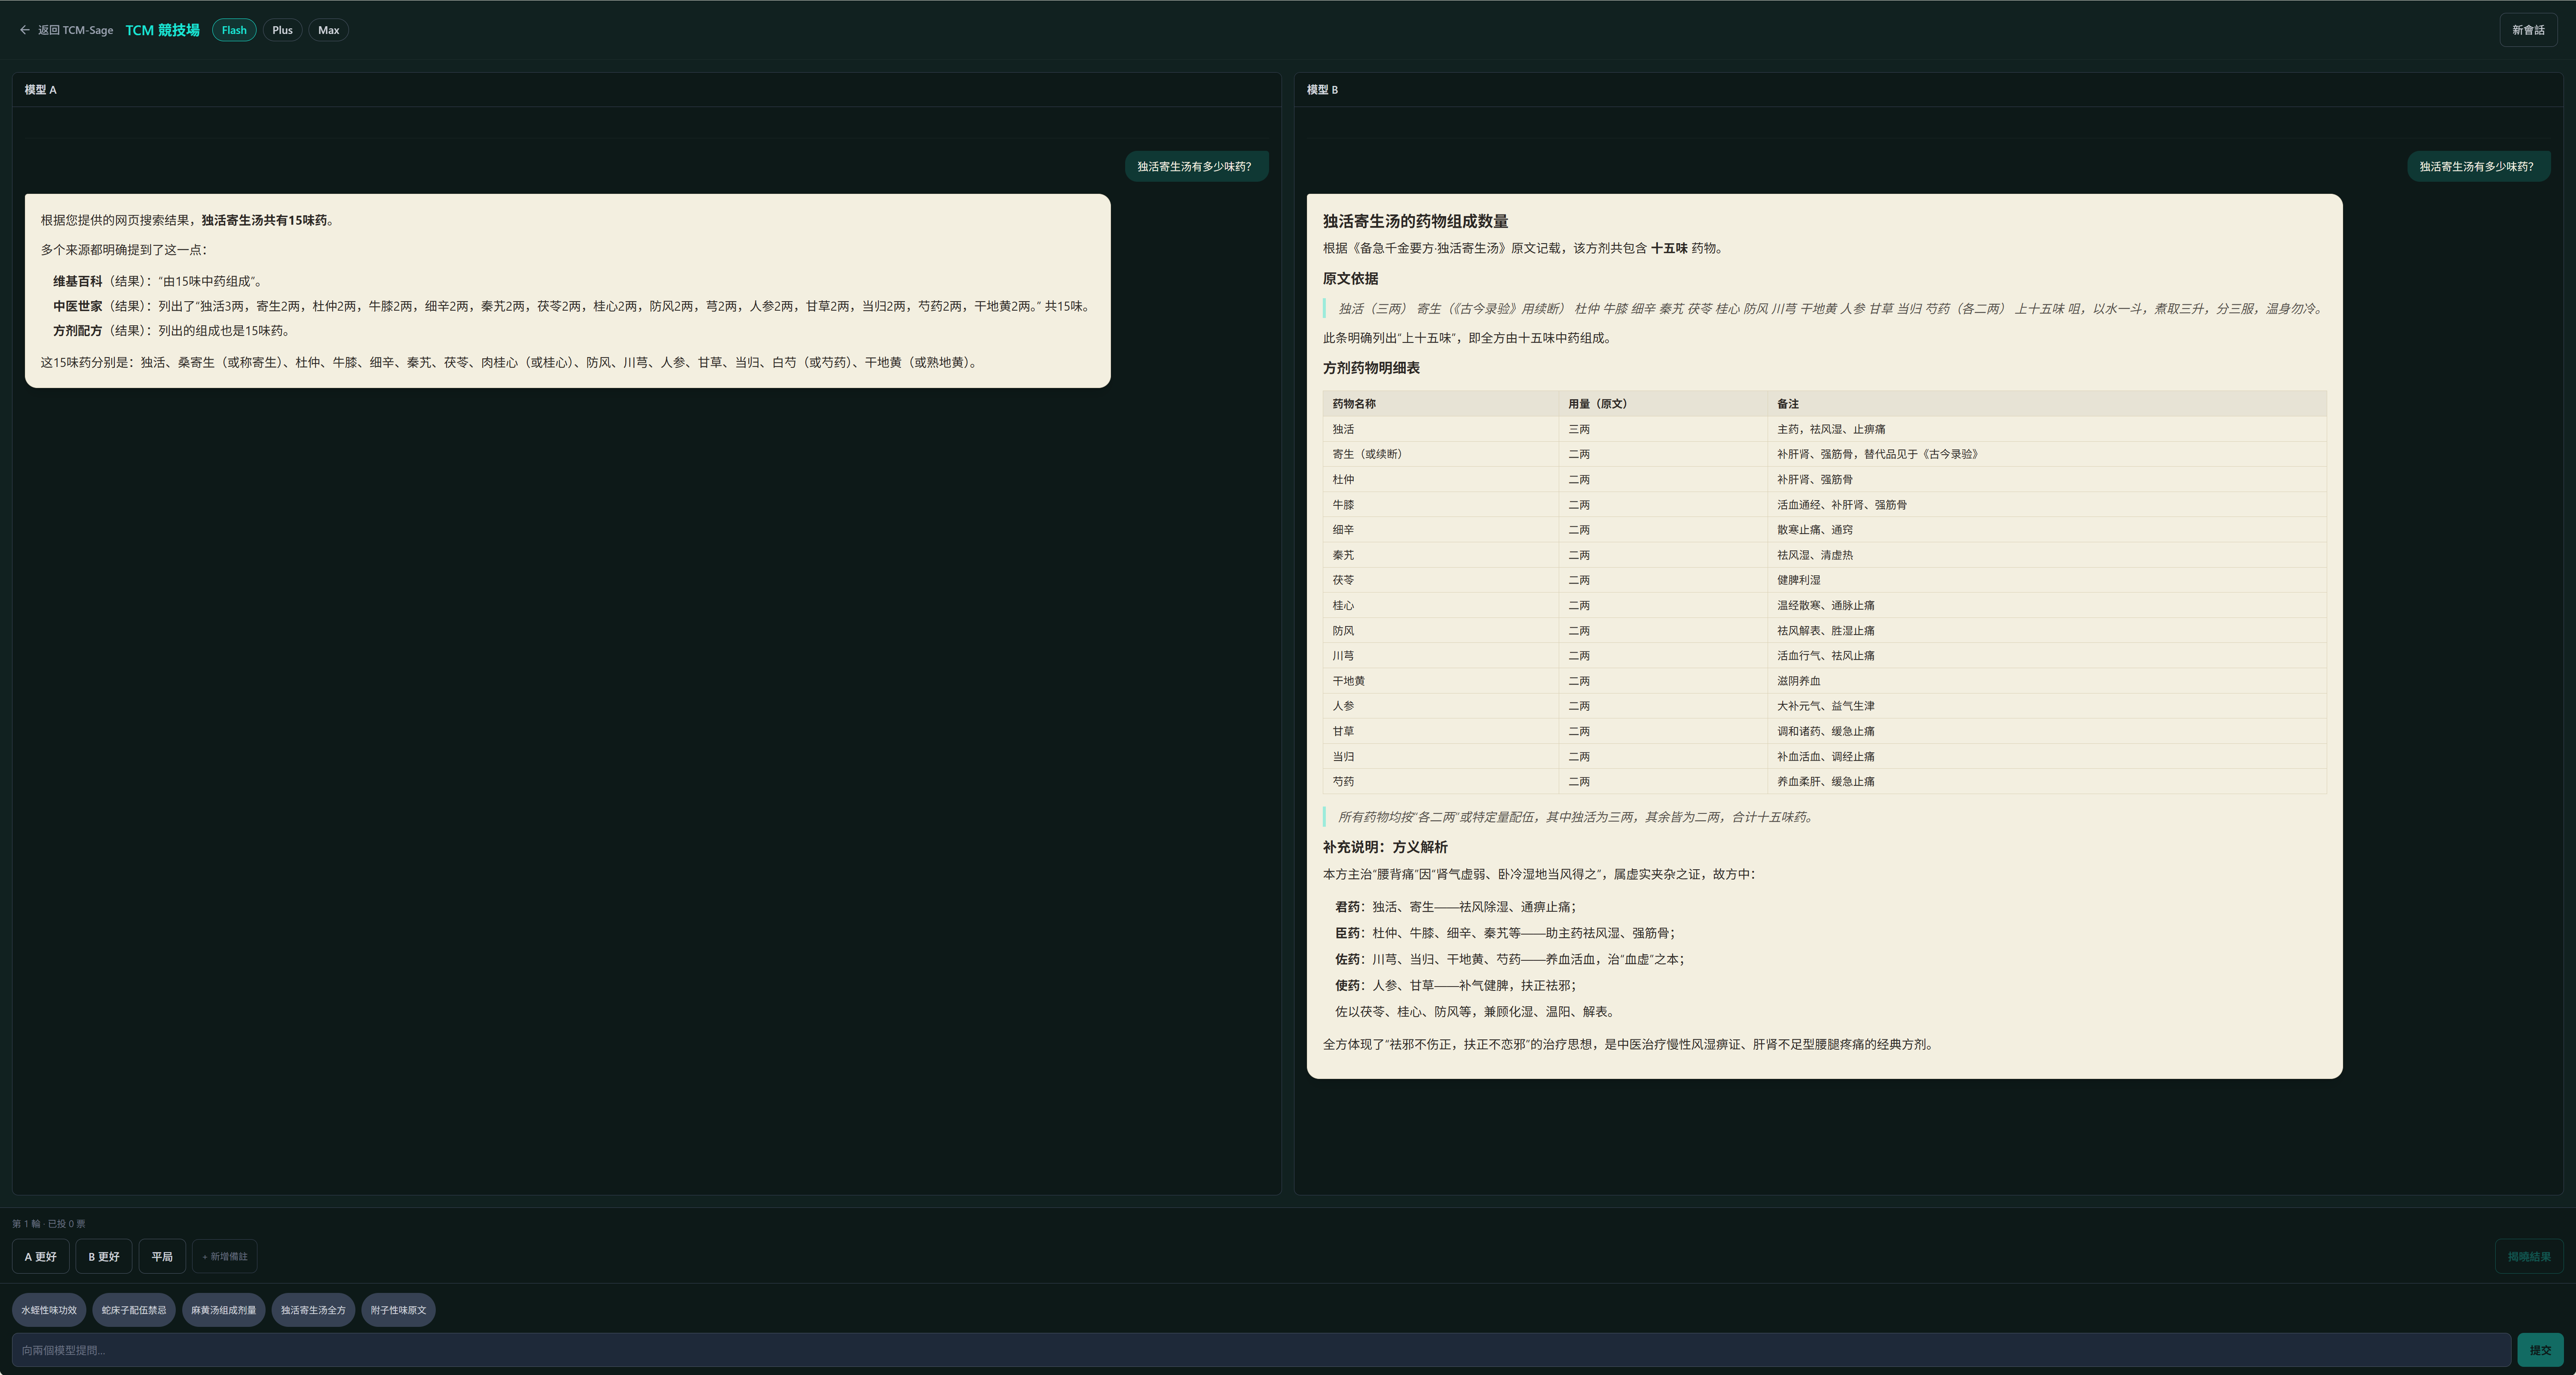
\includegraphics[width=\textwidth]{figures/ui-arena.png}
\caption{The Arena blind A/B evaluation interface with two simultaneous response streams.}
\label{fig:ui_arena}
\end{figure}

\begin{figure}[H]
\centering
\begin{minipage}{0.48\textwidth}
    \centering
    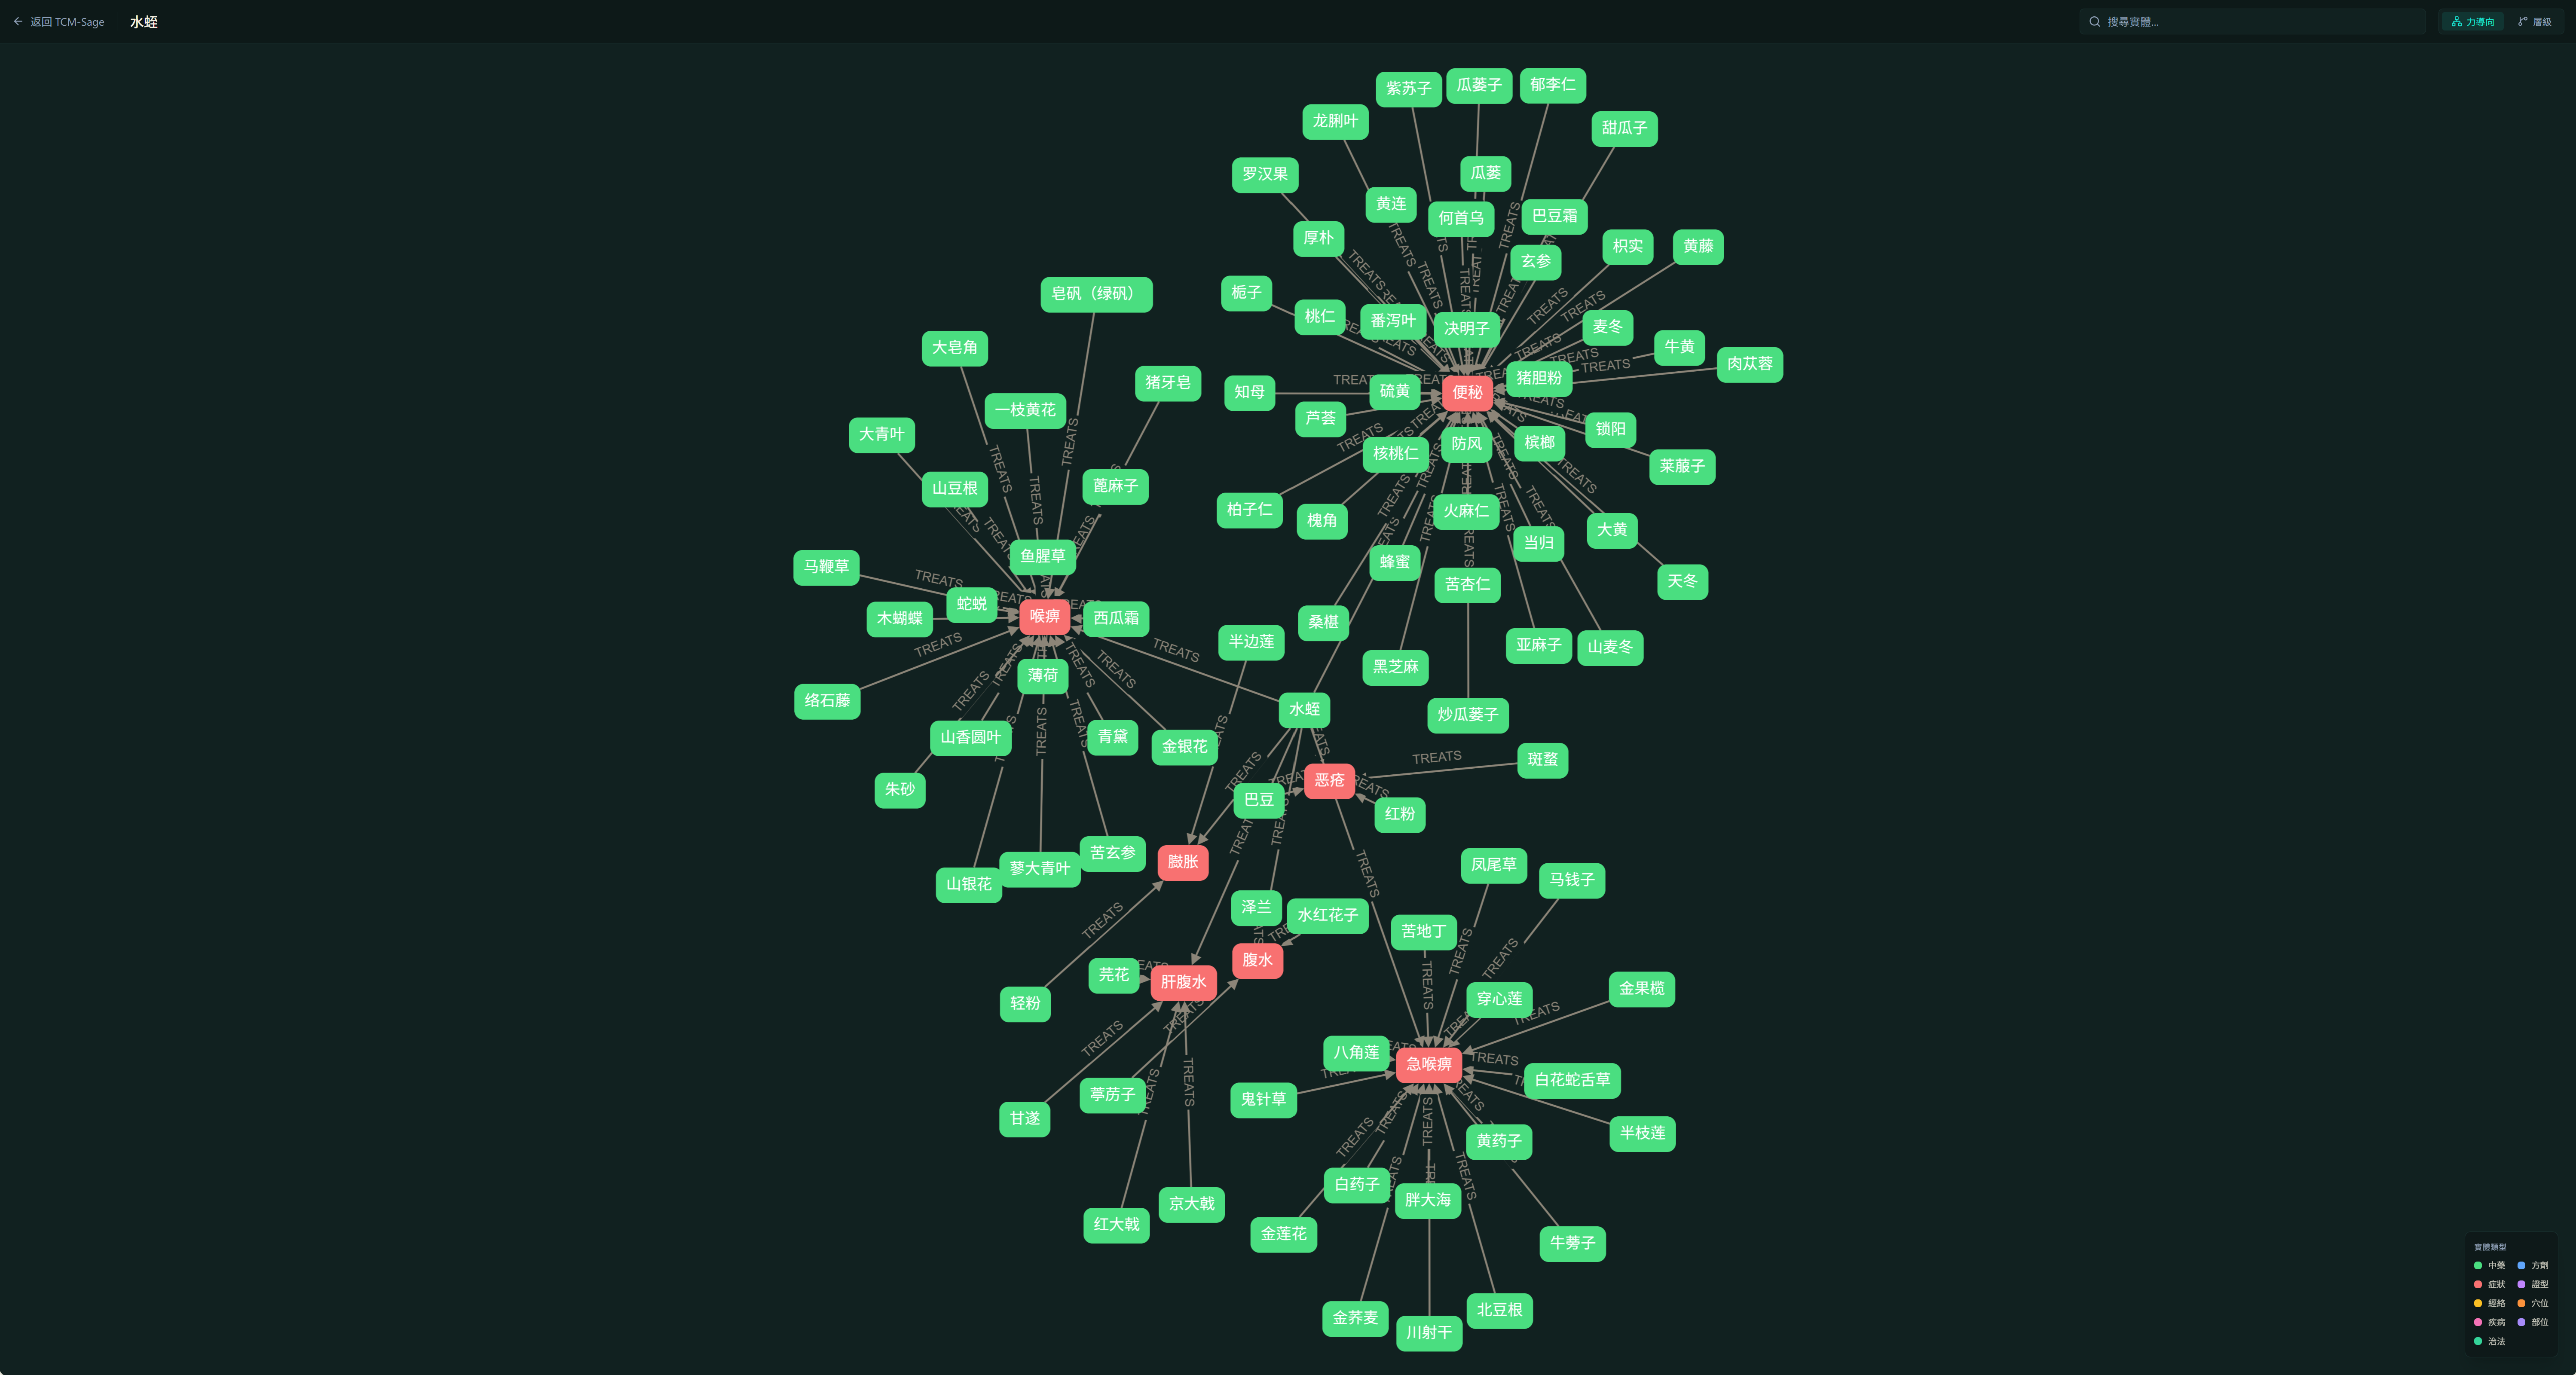
\includegraphics[width=\textwidth]{figures/ui-kg-explorer.png}
    \caption{Full-page Knowledge Graph explorer with entity search and click-to-expand.}
    \label{fig:ui_kg}
\end{minipage}\hfill
\begin{minipage}{0.48\textwidth}
    \centering
    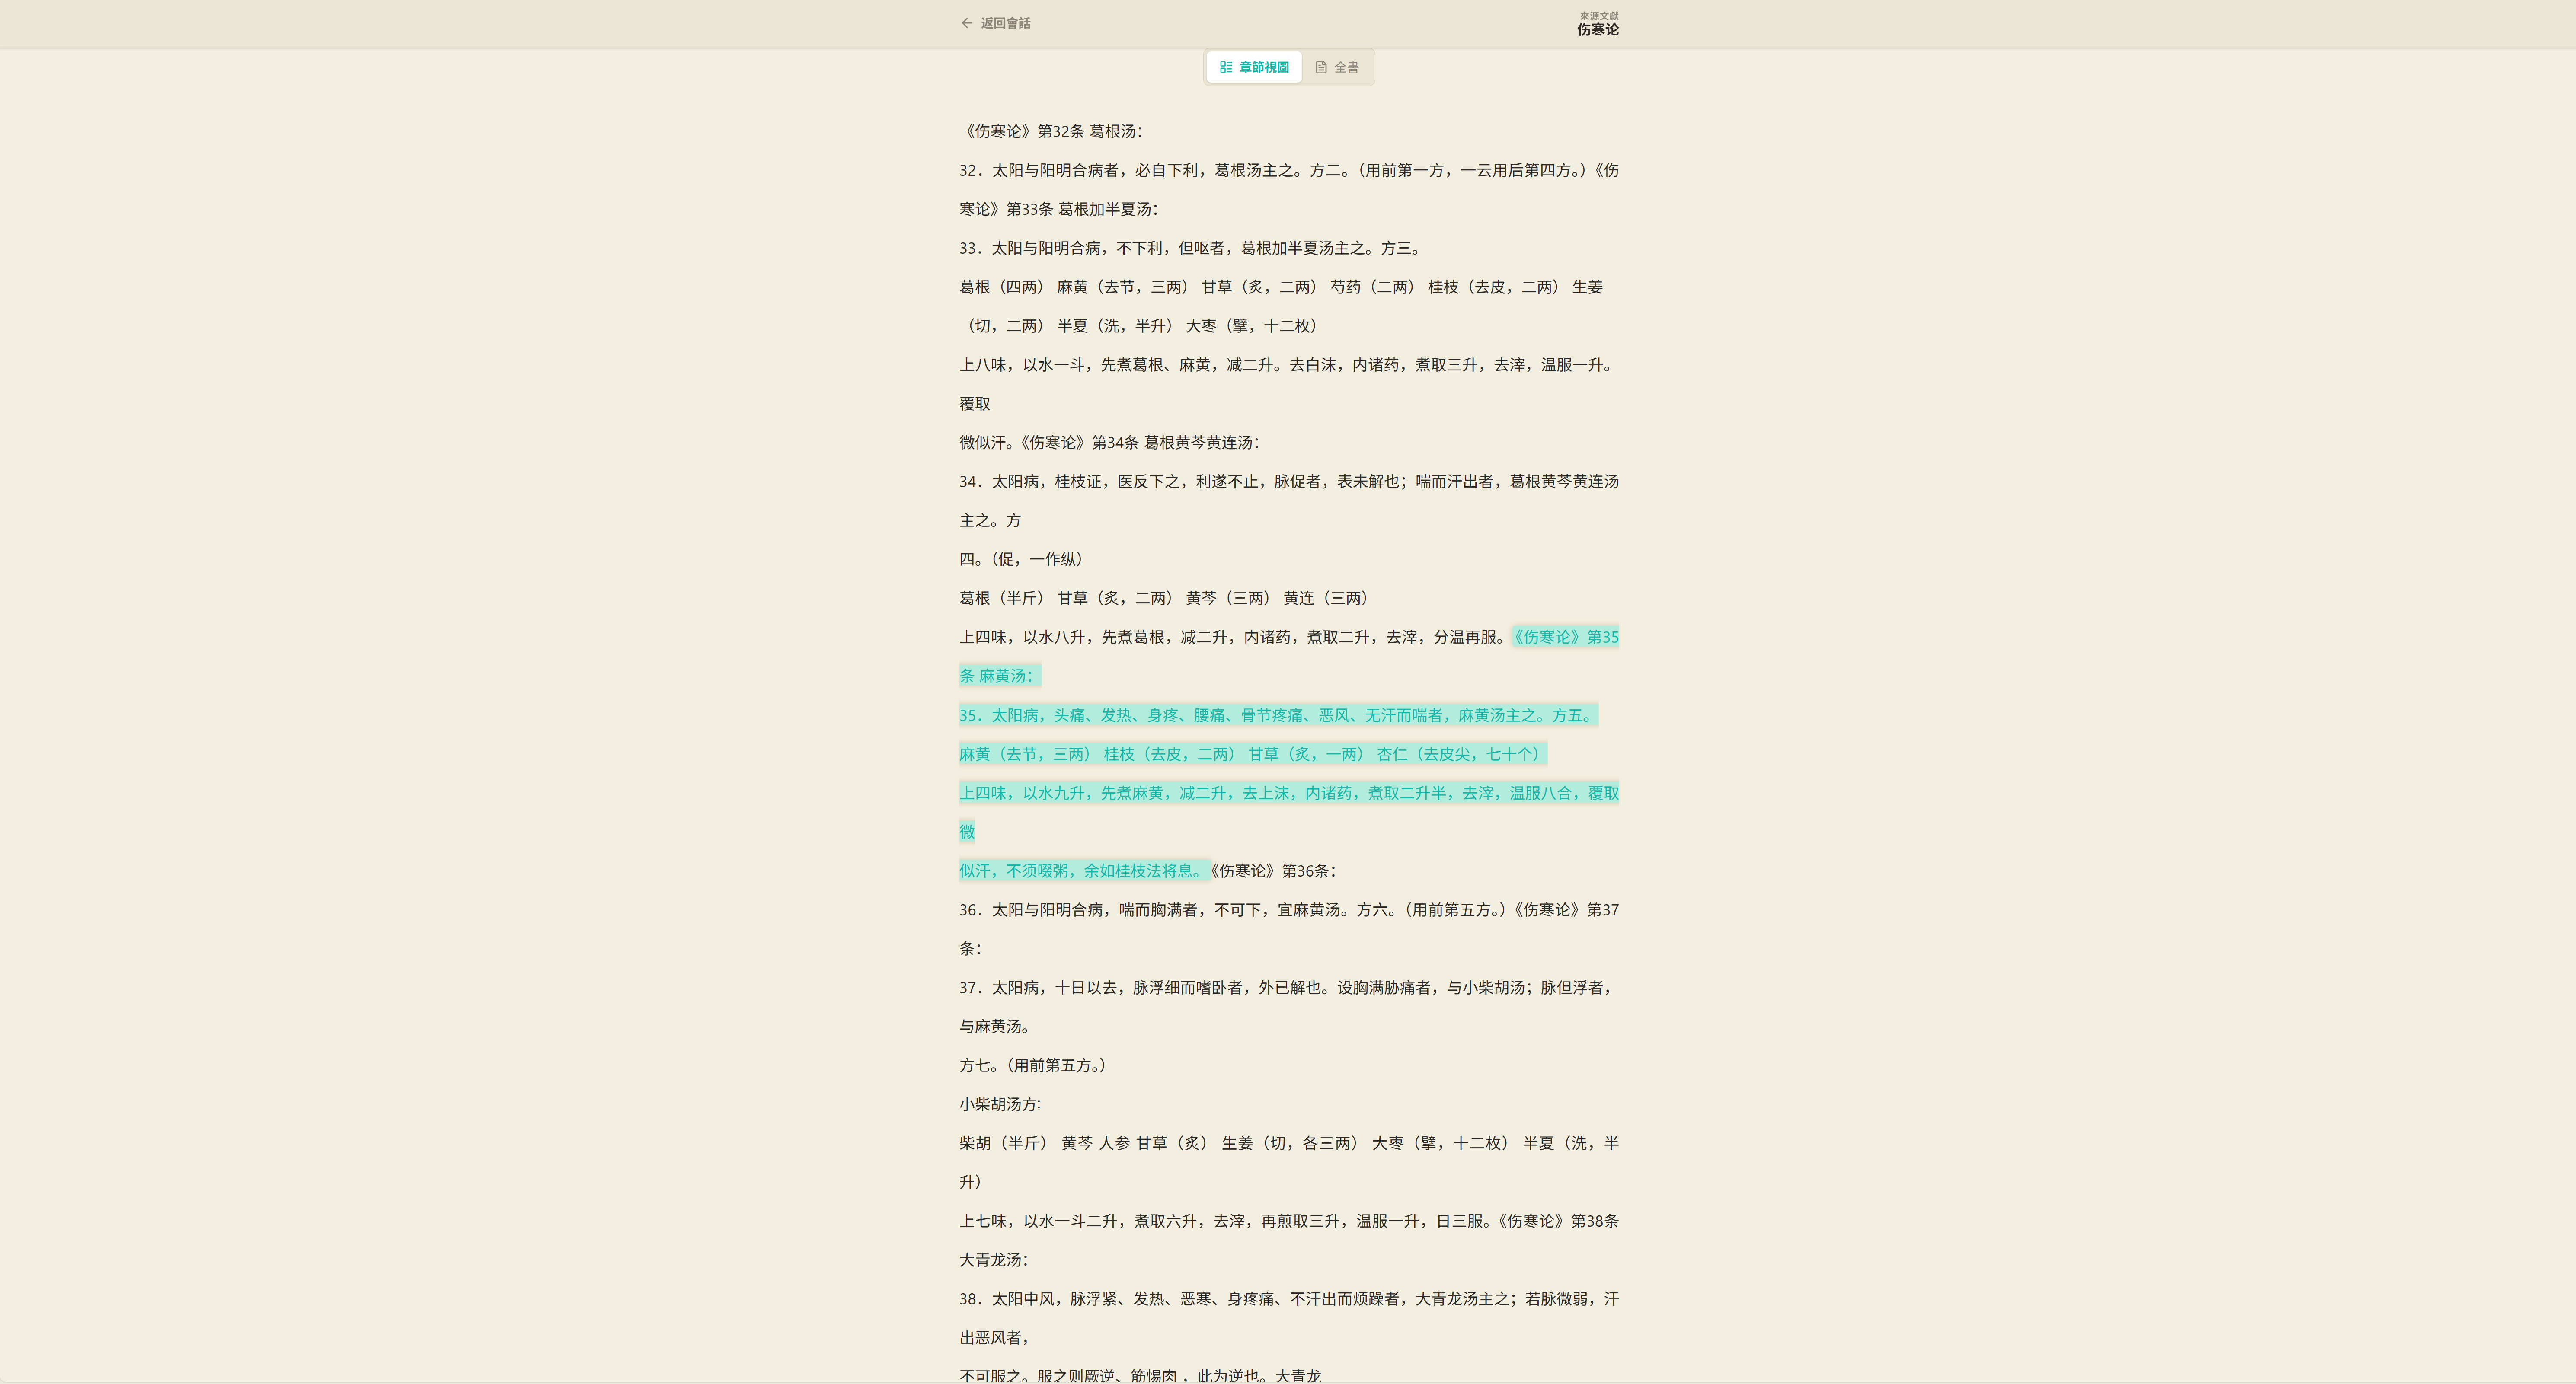
\includegraphics[width=\textwidth]{figures/ui-full-text.png}
    \caption{Full source text viewer showing the original classical passage with metadata.}
    \label{fig:ui_text}
\end{minipage}
\end{figure}

\begin{figure}[H]
\centering
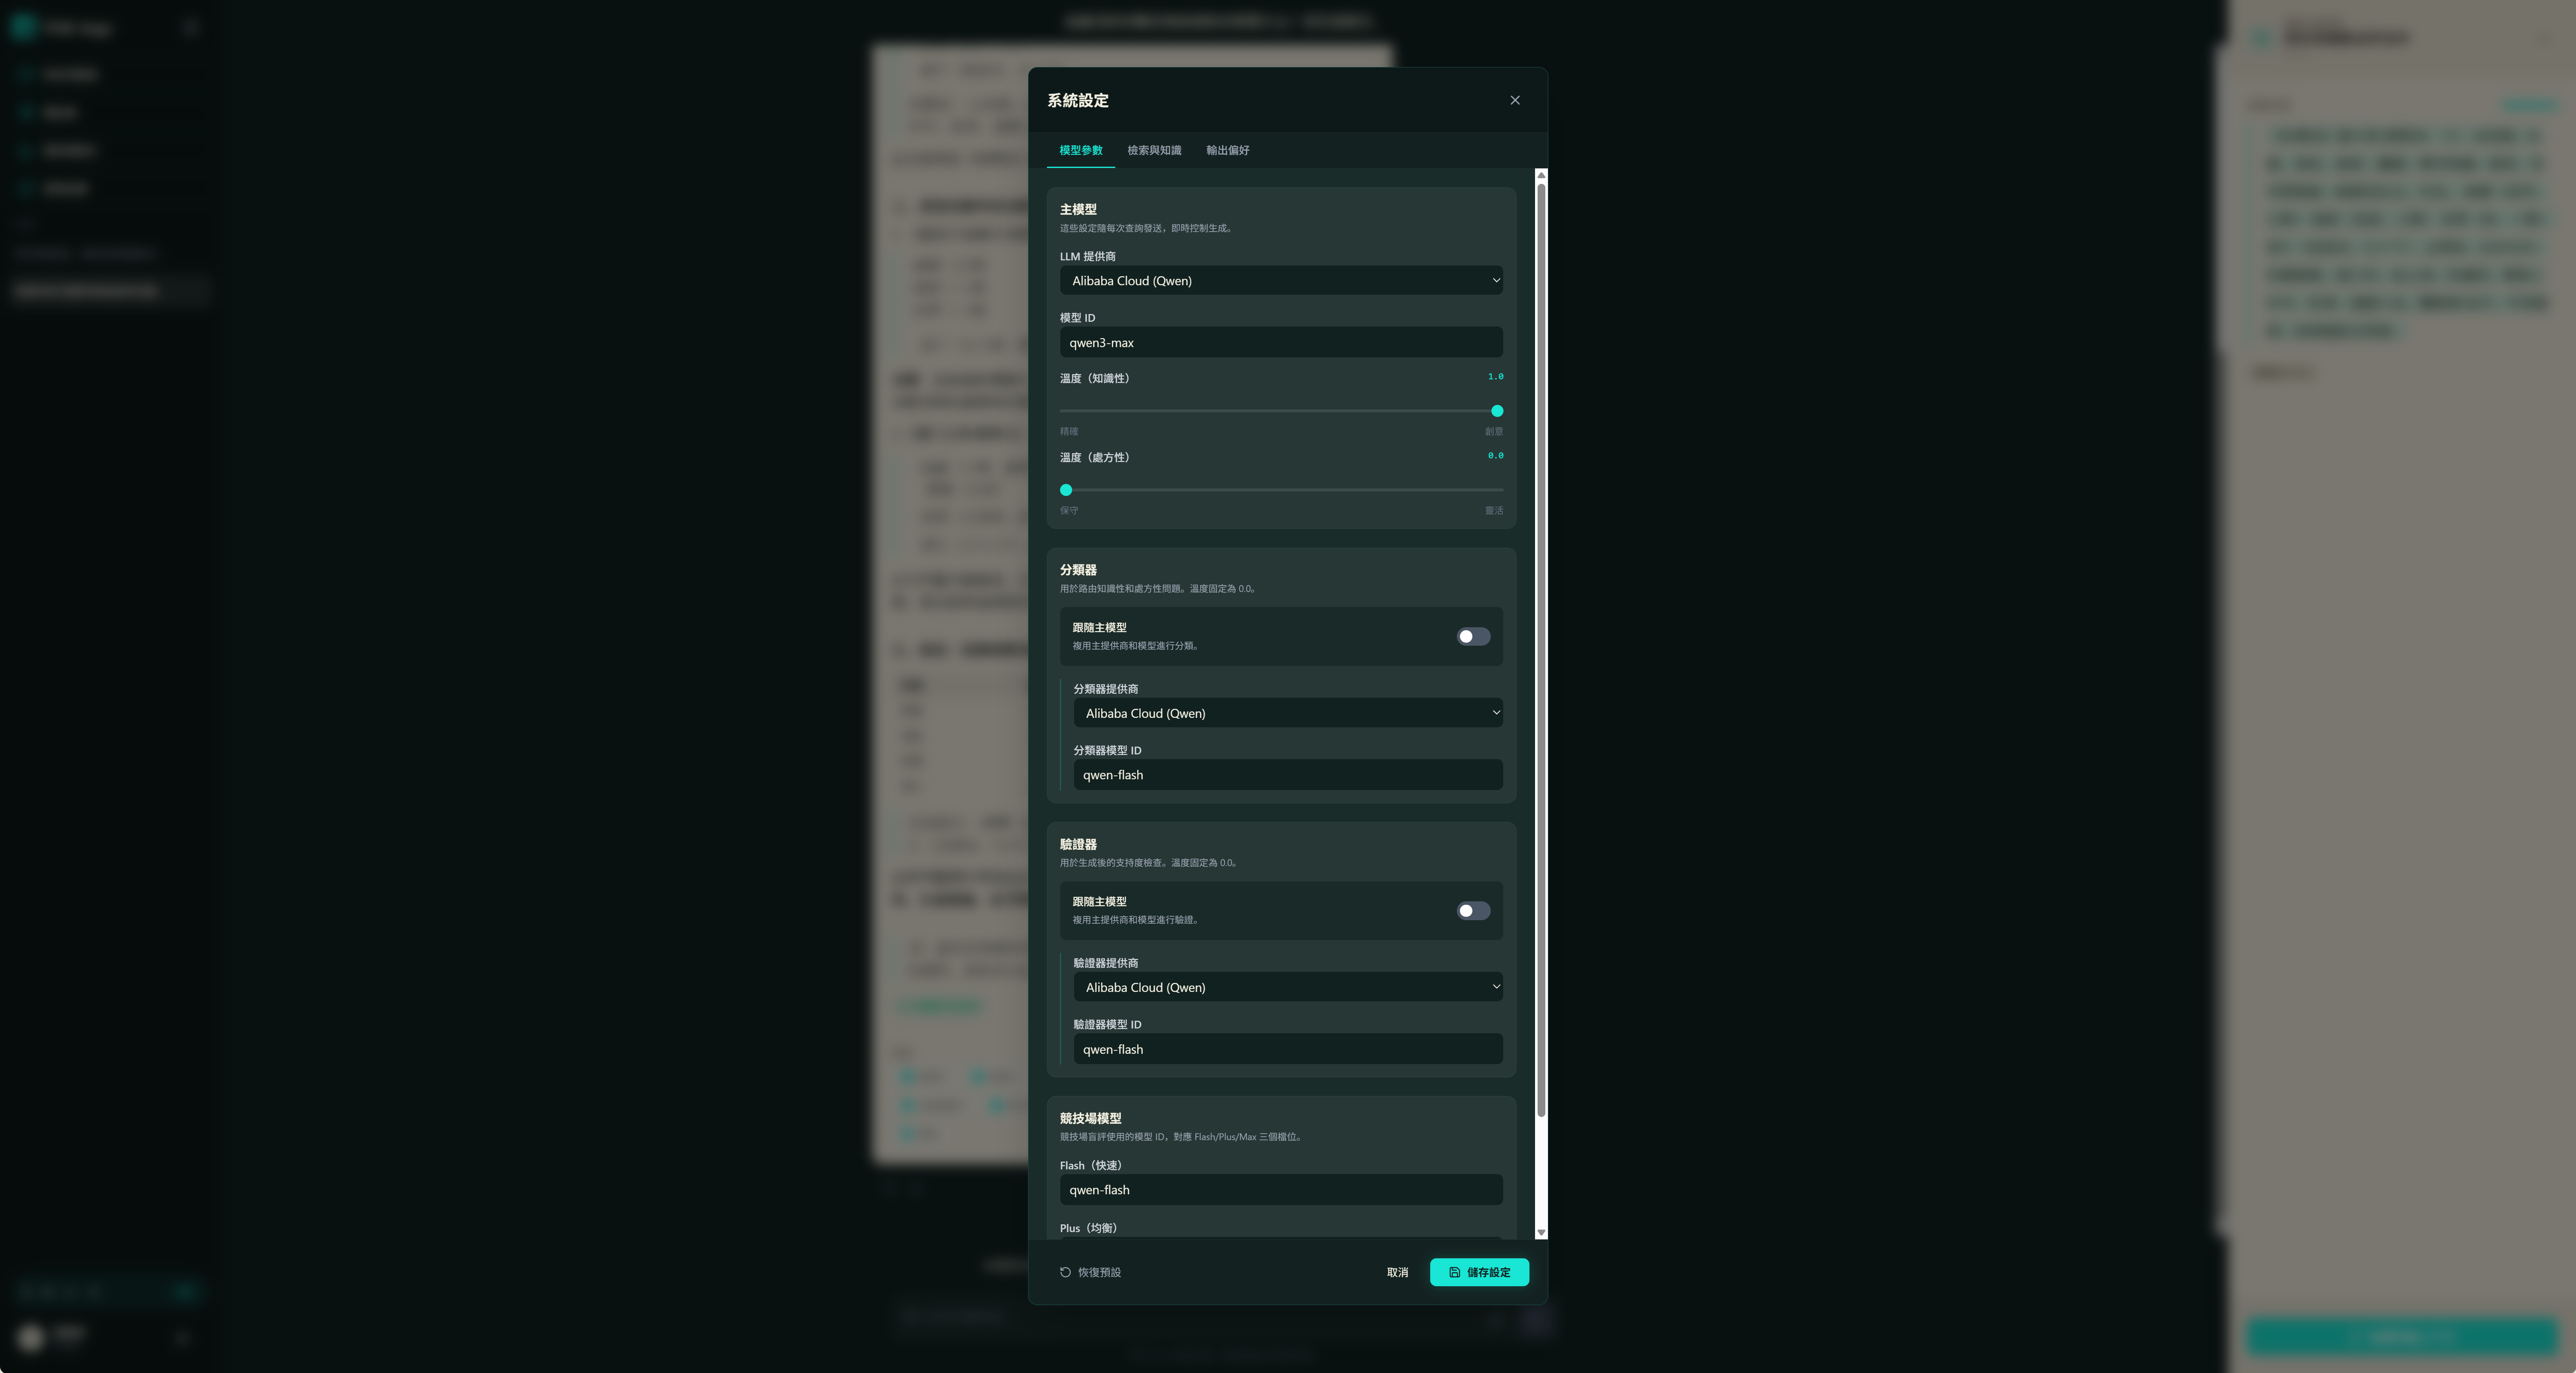
\includegraphics[width=0.5\textwidth]{figures/ui-settings.png}
\caption{The Settings panel allowing configuration of LLM provider, model, and temperature.}
\label{fig:ui_settings}
\end{figure}

\section{Implementation Challenges and Solutions}

\subsection{Retrieval Ranking Bias}
\textbf{Challenge:} Initial testing showed that canonical formula definitions from \textit{Shanghan Lun} were often outranked by lengthy, verbose descriptions in later Ming Dynasty texts (e.g., \textit{Qianjin Fang}), which contained more keyword matches.
\textbf{Solution:} We implemented \textit{Formula-Aware Canonical Retrieval} combined with the \textit{Source Authority Boost}. This ensured that primary sources are always prioritized regardless of their relative brevity compared to later commentaries.

\subsection{RAG Context Engineering}
\textbf{Challenge:} Models like \textit{Qwen-turbo} often ignored formatting rules when the retrieved context exceeded 2,000 characters.
\textbf{Solution:} We adopted "Post-context anchoring," moving the formatting instructions to the very end of the prompt, and utilized \textit{Pattern Priming} by styling the context as Markdown to implicitly guide the model's output structure.

\subsection{Diagnostic Over-Assertion}
\textbf{Challenge:} Early versions of the system would provide definitive diagnoses (e.g., "You have Spleen Deficiency"), which is clinically irresponsible.
\textbf{Solution:} We integrated \textit{Hedging Principles} into the system prompt, requiring the LLM to use uncertain language (e.g., "The symptoms suggest a possibility of...") when evidence is insufficient, and added a mandatory medical disclaimer to all outputs.


\chapter{Evaluation}
\label{ch:evaluation}

This chapter evaluates the efficacy of the TCM-Sage system compared to a non-specialized large language model (LLM) baseline. The evaluation is conducted through a blind A/B testing framework, the "Arena," involving practitioners and students from the Traditional Chinese Medicine (TCM) community.

\section{Experimental Setup}

The evaluation framework was designed to isolate the impact of the specialized RAG (Retrieval-Augmented Generation) pipeline and the TCM-specific system prompt.

\subsection{System Configurations}
Two distinct system configurations were compared:
\begin{enumerate}
    \item \textbf{Treatment (TCM-Sage):} The full pipeline described in Chapter 4, including specialized RAG context from 17 classical texts, SymMap v2.0 knowledge graph integration, and the professional TCM system prompt.
    \item \textbf{Baseline (Plain LLM):} A generic configuration using the same underlying Qwen model but with a "helpful assistant" prompt. To simulate a modern AI's capabilities, the baseline had access to \textbf{DuckDuckGo Web Search} (5 results), representing the current standard for general-purpose retrieval.
\end{enumerate}

\subsection{Blind A/B Design}
A total of 59 votes were collected from a pool of TCM students and practitioners. The evaluation used a blind design:
\begin{itemize}
    \item \textbf{Randomization:} The positions of the Treatment and Baseline responses (A/B) were randomized for each query.
    \item \textbf{Interaction:} Voters entered a clinical or theoretical query and received two simultaneous streams.
    \item \textbf{Metrics:} After reading both responses, voters could select "A is Better," "B is Better," or "Tie." Votes were stored in a JSONL format for statistical analysis.
\end{itemize}

\section{Quantitative Results}

The primary goal of the quantitative analysis was to determine if the TCM-Sage system provided a statistically significant improvement over a general-purpose LLM.

\subsection{Comparative Performance}
The distribution of the 59 votes is summarized below:
\begin{itemize}
    \item \textbf{TCM-Sage Wins:} 38 (64.4\%)
    \item \textbf{Plain LLM Wins:} 15 (25.4\%)
    \item \textbf{Ties:} 6 (10.2\%)
\end{itemize}

The TCM-Sage system outperformed the baseline in over 60\% of cases, more than doubling the win rate of the general-purpose search-augmented model.

\begin{figure}[H]
\centering
\begin{minipage}{0.48\textwidth}
    \centering
    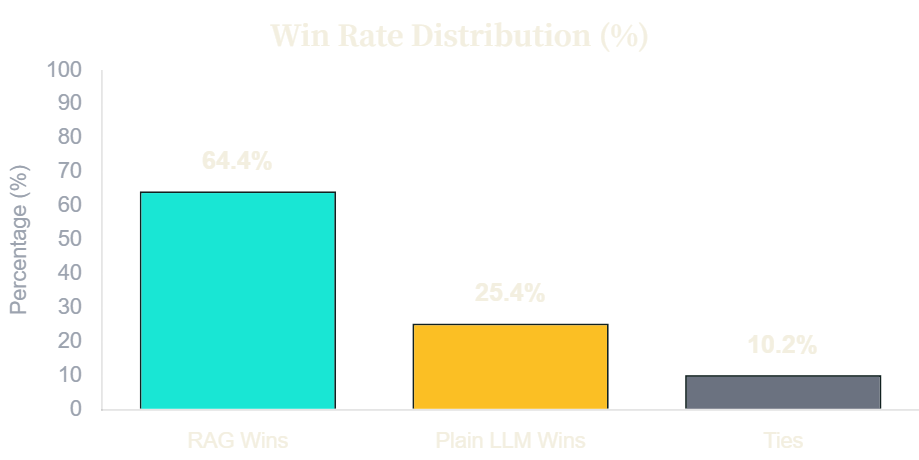
\includegraphics[width=\textwidth]{figures/arena-win-rate.png}
    \caption{Win rate distribution across the three outcomes.}
    \label{fig:winrate}
\end{minipage}\hfill
\begin{minipage}{0.48\textwidth}
    \centering
    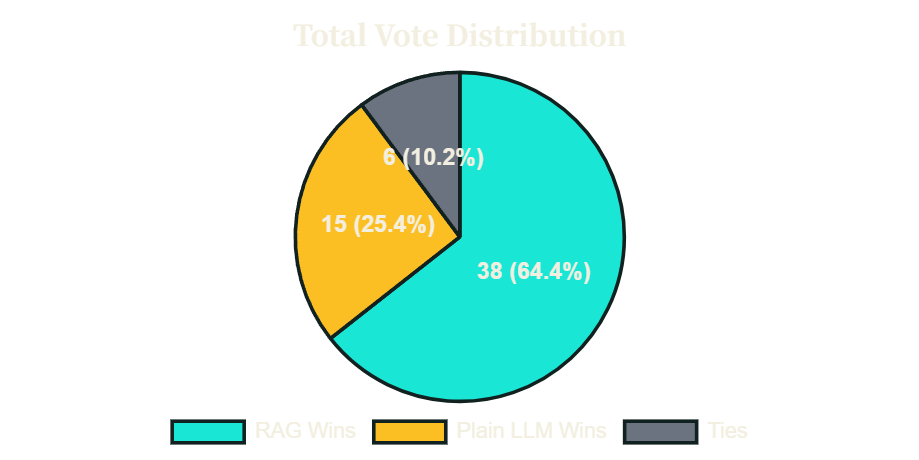
\includegraphics[width=\textwidth]{figures/arena-vote-distribution.png}
    \caption{Total vote distribution (N=59).}
    \label{fig:votedist}
\end{minipage}
\end{figure}

\subsection{Statistical Significance}
To rigorously test the null hypothesis that there is no difference between the two systems, a \textbf{paired t-test} was performed. Each vote was encoded as a paired score: 1 for a TCM-Sage win and 0 for a Plain LLM win (with ties encoded as 0.5 for both). The test evaluated whether the mean paired difference between RAG and plain scores was significantly different from zero.
\begin{itemize}
    \item \textbf{t-statistic:} 3.44
    \item \textbf{p-value:} 0.0011
\end{itemize}
With $p < 0.01$, the results are highly significant, allowing us to reject the null hypothesis.

\subsection{Effect Size}
\textbf{Cohen's d} was calculated to measure the magnitude of the improvement:
\begin{itemize}
    \item \textbf{Cohen's d:} 0.45
\end{itemize}
An effect size of 0.45 indicates a \textit{medium effect}, suggesting that while the general-purpose model is a capable baseline, the specialized TCM-Sage system provides a meaningful and consistent advantage in the quality of clinical reasoning and source accuracy.

\section{Temporal Analysis}

The evaluation was conducted over a four-day period (April 3 to April 6, 2026), during which the system underwent minor iterative refinements based on initial feedback.

\begin{itemize}
    \item \textbf{April 3:} 2 RAG / 1 Plain / 0 Ties (3 votes) --- Initial testing phase.
    \item \textbf{April 4:} 13 RAG / 8 Plain / 6 Ties (27 votes) --- Main testing batch from student groups.
    \item \textbf{April 5:} 8 RAG / 0 Plain / 0 Ties (8 votes) --- Post system prompt and retrieval improvements.
    \item \textbf{April 6:} 12 RAG / 6 Plain / 0 Ties (18 votes) --- Extended testing with a wider group of practitioners.
    \item \textbf{April 7:} 3 RAG / 0 Plain / 0 Ties (3 votes) --- Continued testing.
\end{itemize}

The cumulative trend shows a consistent preference for TCM-Sage, with a notable peak in performance after specific clinical knowledge (e.g., unit conversions) was hard-coded into the system prompt.

\section{Qualitative Feedback and Case Studies}

Qualitative feedback from TCM professionals provided deeper insights into the specific strengths and weaknesses of both systems.

\subsection{Dosage and Unit Conversion}
A doctoral student at Guangzhou University of Chinese Medicine, who also practices at the Guangdong Provincial Hospital of TCM, tested a query regarding the dosage of \textit{Mahuang Tang}. He observed that the general LLM (Baseline), aided by its web search capability, correctly identified the modern unit conversion for Han Dynasty weights. By contrast, the TCM-Sage system at that time provided an incorrect conversion (1 \textit{liang} $\approx$ 3g instead of $\approx$ 13.8g), because the classical texts in the knowledge base do not contain modern unit conversion data.

\textit{Outcome:} This feedback led to the immediate implementation of the \textit{Measurement Conversion} table (1 \textit{liang} $\approx$ 13.8g) in the system prompt. Subsequent tests showed that practitioners found the corrected system far superior to the baseline, as it provided both historical accuracy and modern relevance.

\subsection{Source Traceability}
Students consistently highlighted the \textbf{Citation Panel} as the most valuable feature. One student noted: "The ability to see the original classical text immediately, without having to copy-paste the formula name into a search engine to verify the source, is the key value of this system." This indicates that the \textit{traceability} provided by RAG is as important as the \textit{content} of the generated response.

\subsection{Diagnostic Hedging and Safety}
A doctoral student who also practices as a physician noted that the early version of the system was ``over-assertive'' in its diagnosis of \textit{Pi Xu} (Spleen Deficiency) based on limited symptoms. Following this, \textbf{Hedging Principles} were added to the prompt, requiring the system to use more tentative language (``The symptoms suggest a possibility of...'') when data is incomplete. The practitioner later confirmed that the updated responses felt more like a professional consultation than a ``black-box'' diagnosis.

\subsection{Novel Clinical Insights}
In one recorded case, a student consulted the system for a sore throat. The system suggested \textit{Jiegeng Tang}, a classical formula the student had not considered. Upon reviewing the provided citations, the student confirmed the validity of the recommendation. This demonstrates the system's potential as a "clinical co-pilot" that can surface relevant but overlooked classical knowledge.

\section{Limitations of Evaluation}

While the results are statistically significant, several limitations must be acknowledged:
\begin{enumerate}
    \item \textbf{Sample Size:} 59 votes are sufficient for statistical significance but do not represent a comprehensive clinical trial.
    \item \textbf{Voter Demographic:} The majority of voters were TCM students rather than senior clinicians with decades of experience.
    \item \textbf{Evaluation Format:} The Arena tests overall user preference, which includes factors like formatting and tone, not just clinical accuracy.
    \item \textbf{Prompt Influence:} Because the system prompts differed between the two models, the evaluation measures the effectiveness of the \textit{entire pipeline} (Prompt + RAG + KG), not just the retrieval component in isolation.
\end{enumerate}

\section{Discussion of Results}

The results of the evaluation demonstrate that a specialized RAG system tailored for TCM significantly outperforms a general-purpose search-augmented LLM.

\begin{itemize}
    \item \textbf{Accuracy vs. Verifiability:} The primary advantage of TCM-Sage lies in its ability to provide verbatim classical citations. While the general LLM can often ``summarize'' TCM knowledge from the web, it frequently hallucinates formula origins or misinterprets classical syntax.
    \item \textbf{The Value of Domain Knowledge:} The integration of a specialized knowledge graph and a professional system prompt (including ancient-to-modern measurement conversions) is essential for clinical utility. Without these, even a high-quality RAG system is prone to fundamental errors in interpretation.
    \item \textbf{Impact on the Field:} The $p = 0.0011$ result strongly suggests that specialized AI tools can provide a higher standard of information for the TCM community than general-purpose assistants, particularly in the areas of citation traceability and classical methodology adherence.
\end{itemize}


\chapter{Discussion and Contributions}

\section{Comparison with Existing TCM AI Systems}

TCM-Sage occupies a distinct position in the TCM AI landscape. While existing products pursue an ``AI Doctor'' paradigm, TCM-Sage functions as an evidence-synthesis reference tool. This distinction is not merely semantic; it reflects fundamentally different design philosophies with practical consequences.

General-purpose LLMs such as ChatGPT and Qwen operate as black boxes. When queried about TCM topics, they generate responses from parametric memory without any mechanism for source verification. A practitioner receiving a formula recommendation from ChatGPT cannot determine whether that recommendation originates from \textit{Shanghan Lun}, from a modern textbook, or from the model's interpolation of training data. In clinical contexts where incorrect dosage or formula selection carries real risk, this unverifiability is the primary obstacle to adoption, not hallucination per se.

Specialized TCM AI products have attempted to address domain accuracy but not transparency. HuatuoGPT achieved state-of-the-art results on multiple medical benchmarks \cite{huatuogpt2023}. Qihuang 2.0 (Shuzhi Qihuang), a 32-billion-parameter multimodal model \cite{qihuang2024ecnu}, scored 88.1\% on the TCM licensing examination and incorporated tongue and pulse image analysis. iFlytek's TCM assistant was deployed across primary care institutions in Anhui Province \cite{iflytek2024cnr}. These systems share a common ``AI Doctor'' design philosophy, focusing on direct diagnosis and prescription. TCM-Sage takes a fundamentally different direction: evidence synthesis with traceable citations from classical texts.

TCM-Sage addresses these barriers through five design decisions:

\begin{enumerate}
    \item \textbf{Citation Traceability}: Every claim links to a specific classical text passage, visible through the Citation Panel. Practitioners can verify sources without copy-pasting text into external search tools.
    \item \textbf{Classical Text Specialization}: The 17-text corpus provides depth in foundational TCM theory that general LLMs cannot match, backed by clause-level retrieval for structured texts.
    \item \textbf{Full Local Deployment}: The entire pipeline, including embedding models and LLM inference, can run on consumer hardware via Ollama or LMStudio. No patient data leaves the institution's network.
    \item \textbf{Modular Knowledge Base}: Adding or removing knowledge sources requires only text ingestion, not model retraining. When practitioners suggested adding modern clinical texts during testing, the response was immediate: the architecture supports this without modification.
    \item \textbf{Ancient Measurement Accuracy}: An embedded conversion table provides historically verified unit conversions (Han dynasty \textit{liang} $\approx$ 13.8g, not the commonly misquoted 3g), preventing dosage calculation errors that other systems produce.
\end{enumerate}

The SymMap v2.0 knowledge graph deserves specific mention. Unlike the classical texts, SymMap is a modern pharmacological database integrating contemporary research. The crosswalk bridge connects these modern entities to classical terminology, creating a bidirectional link between historical medical knowledge and current pharmacological understanding. This hybrid of classical texts and modern knowledge graph is unique among TCM AI systems.

\section{Strengths Demonstrated}

The Arena evaluation provides quantitative evidence: with $p = 0.0011$ and Cohen's $d = 0.45$, the preference for TCM-Sage over the baseline is statistically significant at the 1\% level with a medium effect size. This result was observed across five days of testing with different tester groups.

Qualitative feedback reinforced specific strengths. A TCM student consultant summarized four key advantages observed during extended testing:

\begin{enumerate}
    \item \textbf{Focused, relevant responses:} The system provides adequately elaborated answers with valid arguments while avoiding irrelevant details. Unlike general LLMs that tend to produce verbose, unfocused responses mixing TCM with Western medicine or unrelated topics, TCM-Sage stays within the classical framework.
    \item \textbf{Credible source extraction and integration:} The system extracts and integrates credible sources directly from TCM classics, presenting them alongside the generated response through the Citation Panel.
    \item \textbf{TCM-perspective clinical guidance:} The system guides practitioners in thinking from TCM perspectives, including \textit{Materia Medica} recommendations and treatment approach demonstrations grounded in classical methodology (\textit{Bian Zheng Lun Zhi}).
    \item \textbf{Practitioner-informed tuning:} The system prompt and retrieval pipeline were iteratively refined based on feedback from TCM students, resulting in output that aligns with how practitioners expect clinical information to be structured.
\end{enumerate}

The Citation Panel received the strongest individual endorsement, with testers describing it as eliminating the need to manually verify AI-generated claims against source texts. In one case, the system recommended \textit{Jiegeng Tang} (Platycodon Decoction) for a sore throat that the consulting student had not considered. Upon review, he confirmed this as a valid and potentially superior approach from a classical perspective, demonstrating the system's ability to surface overlooked classical formulas.

The modular architecture received indirect validation when practitioners at Guangdong Provincial Hospital of TCM suggested expanding the corpus to include modern clinical masters' works (Zhang Xichun's \textit{Yi Xue Zhong Zhong Can Xi Lu}, Shi Xuemin's acupuncture texts, and Dong's Extraordinary Points system). The fact that such expansion is architecturally straightforward confirms that the design decision to use RAG over fine-tuning was sound.

\section{Limitations and Honest Assessment}

Several limitations emerged during testing and must be acknowledged.

\textbf{Knowledge Boundary Errors.} The system's accuracy is bounded by its corpus. When a practitioner asked about \textit{Mahuang Tang} dosage, the system stated that one Han dynasty \textit{liang} equals approximately 3 grams, a significant error (the correct value is 13.8--15.6g based on archaeological evidence). This occurred because the classical texts contain dosage ratios but not modern unit conversions. The plain LLM baseline, with access to web search, retrieved the correct conversion. This limitation was addressed by embedding a historically verified measurement conversion table directly into the system prompt.

\textbf{Corpus Coverage Gaps.} The 17-text corpus covers foundational theory, \textit{Shanghan}/\textit{Wenbing}, herbology, formulary, and acupuncture. It does not cover surgery, orthopedics, ophthalmology, specialized gynecology or pediatrics texts, or pulse diagnosis monographs. Practitioner feedback was direct: ``These texts are too traditional. Real clinical learning requires modern clinical masters' experience and knowledge systems.'' This feedback, while critical, validates the system's modular design as the appropriate architecture for iterative corpus expansion.

\textbf{Diagnostic Over-Assertion.} The system initially presented diagnostic interpretations with excessive confidence. When analyzing a pediatric case, it concluded \textit{Pi Xu} (spleen deficiency) without sufficient evidence in the case data, and classified an initial rash presentation as \textit{Re Yu Yu Ying} (heat trapped in the nutritive level) when the clinical presentation better supported \textit{Xie Qi Zai Biao} (pathogen at the exterior). Hedging principles were added to the system prompt to mitigate this tendency, but the underlying challenge of calibrating LLM confidence in medical reasoning remains partially unresolved.

\textbf{Evaluation Scale.} The 59-vote Arena sample, while statistically sufficient for significance testing, represents a limited evaluator pool. Most voters were TCM students rather than senior practitioners. The Arena format measures overall preference but does not decompose quality into specific dimensions such as citation accuracy, diagnostic reasoning, or readability.

\section{Ethical Considerations}

TCM-Sage is positioned as an evidence reference tool, not a diagnostic system. This distinction carries ethical weight. The system does not claim to diagnose, and its outputs carry an explicit disclaimer that all suggestions are for clinical reference only, with final diagnostic and prescriptive authority belonging to licensed practitioners.

Data privacy is addressed architecturally. Full local deployment eliminates the need to transmit patient data to external servers. During testing, practitioners at Guangdong Provincial Hospital of TCM noted this as a meaningful advantage, given institutional policies restricting patient data sharing with cloud AI services.

The use of AI tools in developing this project is disclosed in the Acknowledgments section, in compliance with university policy.

\begin{table}[H]
\centering
\caption{Feature comparison between TCM-Sage and existing TCM AI systems.}
\label{tab:comparison}
\begin{tabularx}{\textwidth}{lXXXX}
\toprule
\textbf{Feature} & \textbf{TCM-Sage} & \textbf{HuatuoGPT} & \textbf{Qihuang 2.0} & \textbf{iFlytek TCM} \\
\midrule
Primary Approach & Evidence synthesis & AI Doctor (diagnosis) & AI Doctor (multimodal) & AI Doctor (primary care) \\
Citation Traceability & Clause-level, click-through & None reported & None reported & None reported \\
Knowledge Base & 17 classical texts + SymMap KG & Fine-tuned on medical corpus & TCM KG + tongue/pulse images & Expert KG + clinical data \\
Local Deployment & Full local (LLM + embedding) & Cloud only & Cloud only & Cloud only \\
Knowledge Update & Add text files, re-ingest & Retrain model & Retrain model & Retrain model \\
Evaluation & Arena blind A/B ($p=0.0011$) & Medical benchmark SOTA & TCM licensing exam (88.1\%) & 9,800+ assisted diagnoses \\
\bottomrule
\end{tabularx}
\end{table}


\chapter{Conclusion and Future Work}

\section{Summary of Contributions}

This project developed TCM-Sage, a working evidence-synthesis system for classical Traditional Chinese Medicine texts. The system addresses a gap that neither general-purpose LLMs nor existing TCM AI products fill: transparent, citation-backed retrieval from classical medical literature with source traceability.

The principal technical contributions are:

\begin{enumerate}
    \item \textbf{Hybrid RAG Pipeline for Classical Chinese}: A retrieval pipeline combining DashScope text-embedding-v4 (1024 dimensions) vector search with SymMap v2.0 knowledge graph traversal. The crosswalk bridge maps modern medical terminology to classical Chinese entities, addressing the semantic drift that spans two millennia of medical writing.

    \item \textbf{Domain-Specific Retrieval Optimizations}: Formula-aware canonical retrieval ensures that queries about classical formulas (e.g., \textit{Mahuang Tang}) return results from their canonical source texts first. Source authority boosting applies topic-dependent chronological weighting. Clause-level chunking preserves the natural semantic units of structured texts such as \textit{Shanghan Lun} (388 clauses) and \textit{Jingui Yaolue} (489 clauses).

    \item \textbf{RAG Context Engineering}: The discovery of Pattern Priming --- that formatting retrieved context as markdown causes the LLM to mirror markdown in its output --- and post-context instruction anchoring, where formatting directives placed after retrieved passages maintain effectiveness despite the ``lost-in-the-middle'' attention pattern.

    \item \textbf{Arena Blind A/B Evaluation}: A dual-streaming evaluation system inspired by the LMSYS Chatbot Arena, with paired t-test and Cohen's $d$ validation. Results from 59 votes yielded $p = 0.0011$ and $d = 0.45$, establishing statistically significant preference for the RAG system over a general LLM with web search.

    \item \textbf{Practitioner Validation}: Testing by TCM students and doctoral candidates at Guangzhou University of Chinese Medicine (several of whom also practice at Guangdong Provincial Hospital of TCM) confirmed the system's clinical utility for evidence retrieval. The Citation Panel was identified as the primary value differentiator, and the system demonstrated the ability to surface classical formulas that practitioners had not considered.
\end{enumerate}

\section{Future Work}

Practitioner feedback during testing defined a clear development roadmap. The following directions are ordered by priority and feasibility.

\subsection{Corpus Expansion}

The most consistent feedback was that the current 17-text corpus, while strong in classical theory, lacks modern clinical practice material. Specific texts recommended by practitioners include:

\begin{itemize}
    \item \textbf{Modern clinical masters}: Zhang Xichun's \textit{Yi Xue Zhong Zhong Can Xi Lu} (a foundational text for Chinese-Western integrated medicine), works by Liu Duzhou and Feng Shilun (classical formula specialists), and Zhang Jingyue's \textit{Jingyue Quanshu}.
    \item \textbf{Modern acupuncture}: Shi Xuemin's \textit{Shi Yong Zhen Jiu Xue} (evidence-based stroke treatment protocols), Dong's Extraordinary Points system, Cheng Dan'an's \textit{Zhongguo Zhen Jiu Xue} (integrating Western neuroanatomy), and Takeda Ken's \textit{Zhen Jiu Zhen Sui} (Japanese acupuncture).
    \item \textbf{Pharmacology}: \textit{Ben Cao Yao Zheng} for clinical drug evidence.
    \item \textbf{Chinese-Western integration}: Modern clinical pharmacology references to support practitioners who combine both approaches.
\end{itemize}

The modular RAG architecture makes corpus expansion straightforward: new texts require only UTF-8 source files and a single ingestion run. No model retraining is necessary.

\subsection{Platform Development}

A TCM student tester expressed interest in recommending the system to his university's School of Chinese Medicine and exploring case competition entry. This suggests potential for development beyond an individual project into a platform serving TCM education programs. Each institution could maintain its own knowledge base supplemented with course materials, clinical SOPs, and local reference documents.

\subsection{Patient-Friendly Mode}

Practitioners noted that pure TCM terminology is difficult for general audiences to understand. A future mode could provide simplified explanations alongside classical citations, expanding the user base to include patients and health-conscious individuals seeking reliable TCM information.

\subsection{Fine-Tuned Base Model Integration}

The current architecture uses general-purpose Qwen models as the generation backbone. Stacking a TCM-specialized fine-tuned model (such as HuatuoGPT or a custom fine-tune) as the base, with the RAG pipeline providing retrieved context, could yield compounding quality improvements. The RAG architecture explicitly supports this: the base LLM is a configurable component.

\subsection{Expanded Evaluation}

Future evaluation should address the current study's limitations: larger sample sizes, inclusion of senior practitioners as evaluators, and dimension-specific scoring rubrics that separately measure citation accuracy, diagnostic reasoning quality, completeness, and readability. Longitudinal studies tracking system improvement across development iterations would strengthen the evidence base.

\section{Goal Completion}

The original project proposal set out to build ``an explainable, evidence-backed tool'' based on RAG architecture that would function as ``an intelligent clinical reference assistant'' with traceable citations, hybrid retrieval (vector search and knowledge graph), and user acceptance testing with TCM practitioners. The following table summarizes the completion status of each proposed aim:

\begin{table}[H]
\centering
\caption{Proposed aims and completion status.}
\begin{tabularx}{\textwidth}{Xll}
\toprule
\textbf{Proposed Aim} & \textbf{Status} & \textbf{Notes} \\
\midrule
Evidence-synthesis tool, not AI Doctor & Achieved & Core design principle maintained \\
Glass Box citations linked to source text & Achieved & Citation Panel with click-through \\
RAG architecture with hybrid retrieval & Achieved & Vector + KG + reranker \\
Specialized TCM knowledge base & Exceeded & 17 texts (proposal suggested 1) \\
Knowledge graph for terminology bridging & Achieved & SymMap v2.0 (18,450 entities) \\
User acceptance testing with practitioners & Achieved & Arena blind A/B (59 votes, $p=0.0011$) \\
\bottomrule
\end{tabularx}
\end{table}

The evaluation methodology evolved from the initially proposed TCMEval-SDT benchmark and Likert-scale surveys to a blind A/B Arena system with statistical validation, following discussions with the project supervisor. This approach better captures overall system quality as perceived by end users, rather than isolated retrieval metrics.

All core proposed aims have been achieved or exceeded. The system is functional, tested with real practitioners, and statistically validated.

\section{Closing Remarks}

TCM-Sage demonstrates that retrieval-augmented generation is a viable approach for making classical medical literature accessible through modern AI interfaces. The system does not replace human expertise; it provides the evidence base that human experts need to make informed decisions. In a field where the source texts span two thousand years of accumulated clinical wisdom, the ability to search, retrieve, and cite that wisdom accurately and transparently has practical value.

The project began with a straightforward observation: practitioners need better tools for navigating classical texts. It concludes with a working system, statistical evidence of its effectiveness, and a clear roadmap shaped by the practitioners it was built to serve.


% References (handbook position: after final chapter, before appendices)
\bibliographystyle{abbrvnat}
\bibliography{references}

\appendix
\chapter{Classical Text Corpus}

Table~\ref{tab:corpus_detail} provides the complete list of classical TCM texts included in TCM-Sage, with their dynasty of origin, attributed author, chunking strategy, and resulting chunk count.

\begin{table}[H]
\centering
\caption{Detailed corpus breakdown of the 17 classical texts.}
\label{tab:corpus_detail}
\begin{tabularx}{\textwidth}{>{\raggedright\arraybackslash}X>{\raggedright\arraybackslash}l>{\raggedright\arraybackslash}Xrr}
\toprule
\textbf{Text} & \textbf{Dynasty} & \textbf{Author} & \textbf{Chunks} & \textbf{Strategy} \\
\midrule
Bencao Gangmu & Ming & Li Shizhen & 5,169 & Chapter \\
Beiji Qianjin Yaofang & Tang & Sun Simiao & 2,326 & Chapter \\
Rumen Shiqin & Jin & Zhang Congzheng & 920 & Chapter \\
Jingui Yaolue & E. Han & Zhang Zhongjing & 489 & Clause \\
Danxi Xinfa & Yuan & Zhu Zhenheng & 413 & Chapter \\
Shennong Bencao Jing & W. Han & Unknown & 401 & Chapter \\
Shanghan Lun & E. Han & Zhang Zhongjing & 388 & Clause \\
Zhenjiu Jiayijing & W. Jin & Huangfu Mi & 376 & Chapter \\
Lanshi Micang & Yuan & Li Dongyuan & 318 & Chapter \\
Wenbing Tiaobian & Qing & Wu Jutong & 313 & Chapter \\
Huangdi Neijing Suwen & W. Han & Unknown & 295 & Chapter \\
Huangdi Neijing Lingshu & W. Han & Unknown & 227 & Chapter \\
Suwen Xuanji Yuanbing Shi & Jin & Liu Wansu & 205 & Chapter \\
Piwei Lun & Yuan & Li Dongyuan & 158 & Chapter \\
Neiwaishang Bianhuo Lun & Yuan & Li Dongyuan & 95 & Chapter \\
Bashiyi Nanjing & E. Han & Unknown & 88 & Chapter \\
Wenre Lun & Qing & Ye Tianshi & 23 & Chapter \\
\midrule
\textbf{Total} & & & \textbf{12,204} & \\
\bottomrule
\end{tabularx}
\end{table}

\chapter{System Setup and Reproduction Guide}

This appendix outlines the steps required to set up, configure, and run TCM-Sage from the source repository.

\section*{Prerequisites}
\begin{itemize}
    \item Python 3.11+ with \texttt{pip}
    \item Node.js 18+ with \texttt{npm}
    \item A DashScope API key (or alternative LLM provider credentials)
    \item Git
\end{itemize}

\section*{Step 1: Clone and Install}
\begin{verbatim}
git clone https://github.com/AndyZHENG0715/TCM-Sage.git
cd TCM-Sage

# Python backend
python -m venv venv
venv\Scripts\activate          # Windows
source venv/bin/activate      # Unix/macOS
pip install -r requirements.txt

# Frontend
cd web && npm install && cd ..
\end{verbatim}

\section*{Step 2: Configure Environment}
Copy \texttt{.env.example} to \texttt{.env}, then fill in the required API keys and provider settings:
\begin{verbatim}
DASHSCOPE_API_KEY=your_key_here
LLM_PROVIDER=alibaba
\end{verbatim}
See \texttt{docs/CONFIG.md} for the full list of configurable environment variables.

\section*{Step 3: Build the Vector Index}
\begin{verbatim}
venv\Scripts\python src/ingest.py
\end{verbatim}
This step processes the 17 classical texts in \texttt{data/source/}, generates embeddings via DashScope, and stores them in ChromaDB at \texttt{vectorstore/chroma/}. The ingestion pipeline supports checkpointing and resume. Initial ingestion typically takes approximately 30--60 minutes because of API batch limits.

\section*{Step 4: Start the Application}
\begin{verbatim}
# Terminal 1: Backend (port 8000)
venv\Scripts\python src/api.py
# Unix/macOS: python src/api.py

# Terminal 2: Frontend (port 3000)
cd web && npm run dev
\end{verbatim}
Access the application at \texttt{http://localhost:3000}.

\section*{Step 5: Local Deployment (Optional)}
For fully local operation without cloud API calls, install Ollama and set the provider configuration as follows:
\begin{verbatim}
LLM_PROVIDER=ollama
OLLAMA_BASE_URL=http://localhost:11434/v1
\end{verbatim}
The system supports fully local deployment. Both LLM inference and embedding can run on local hardware. The current default uses DashScope cloud APIs for convenience, but substituting a local embedding model in \texttt{src/embeddings.py} and configuring a local LLM provider enables fully offline operation.

\end{document}
